\documentclass[fleqn,10pt]{wlscirep}
\usepackage[utf8]{inputenc}
\usepackage[T1]{fontenc}
\usepackage{multirow, wrapfig, comment, subcaption, graphicx, standalone, pgfplots, tikz, bbm, tabularx, booktabs, siunitx}
\usepackage{enumitem}
\usepackage{xcolor}
\usetikzlibrary{scopes, backgrounds, matrix, shapes.geometric, patterns,
    decorations.markings, arrows.meta, calc, positioning}
\usepgfplotslibrary{fillbetween}

\pgfplotsset{compat=1.18}

\DeclareSIUnit{\dBm}{dBm}

\definecolor{cb_black}{RGB}{0,0,0}
\definecolor{cb_sky_blue}{RGB}{86,180,233}
\definecolor{cb_yellow}{RGB}{240,228,66}
\definecolor{cb_reddish_purple}{RGB}{204,121,167}
\definecolor{cb_vermillion}{RGB}{213,94,0}
\definecolor{cb_blue}{RGB}{2,112,189}
\definecolor{hs_blue}{RGB}{51,51,255}
\definecolor{imu_green}{RGB}{0,255,0}
\definecolor{cb_orange}{RGB}{229,126,34}
\definecolor{cb_green}{RGB}{113,178,112}
\definecolor{cb_dark_gray}{RGB}{102,102,102}
\definecolor{cb_gray}{RGB}{102,102,102}

% Revision-marking macros for the marked-up version. All three are paragraph-safe
% (group + \color form, accept \par). For the clean submission version, redefine
% each to {#1} (see final.tex).
%   \rev   = added or revised text             -> blue
%   \adj   = adjusted numerical value          -> orange
%   \moved = moved but otherwise unaltered     -> magenta
\definecolor{revblue}{RGB}{0,0,200}
\definecolor{revorange}{RGB}{220,120,0}
\definecolor{revmagenta}{RGB}{180,0,160}
\newcommand{\rev}[1]{{\color{revblue}#1}}
\newcommand{\adj}[1]{{\color{revorange}#1}}
\newcommand{\moved}[1]{{\color{revmagenta}#1}}

\newcommand{\legline}[2]{%
    \tikz[baseline=-0.5ex]{
        \draw[#1, #2, line width=1.5pt] (0,0) -- (0.5,0);
    }%
}
\newcommand{\legmark}[2]{%
    \tikz[baseline=-0.5ex]{
        \node[#2, fill=#1, draw=#1, inner sep=2pt, scale=0.8] at (0,0) {};
    }%
}
\newcommand{\circled}[1]{\tikz[baseline=(char.base)]{\node[shape=circle, draw, inner sep=1pt, font=\scriptsize\bfseries, line width=0.5pt] (char) {#1};}}

\pgfplotsset{
    every axis/.append style={
        axis x line=bottom,
        axis y line=left,
        label style={font=\bfseries},
        tick label style={font=\small},
        legend style={font=\small},
        grid=major,
        grid style={dashed, gray!50},
    }
}

\title{Truly Mobile Sub-Terahertz Communications Beyond 6G via Just-in-Time IMU-Assisted Beam Management}
\author[1*]{Sergey Petrushkevich}
\author[2]{Vitaly Petrov}
\author[1]{Josep M. Jornet}
\affil[1]{Northeastern University, Department of Electrical and Computer Engineering \& \newline Institute for the Wireless Internet of
Things, Boston, 02115, MA, USA}
\affil[2]{KTH Royal Institute of Technology, Department of Communications Systems, \newline School of Electrical Engineering and Computer Science, Stockholm, 11428, Sweden}
\affil[*]{Corresponding author, petrushkevich.s@northeastern.edu}

\begin{abstract}
Sub-Terahertz (sub-THz) communication is a candidate technology for beyond-sixth-generation (beyond-6G) wireless networks, promising up to Terabit-per-second data rates and microsecond-level latencies. However, the highly directional sub-THz beams required to overcome severe path loss make maintaining reliable beam alignment under mobility extremely challenging. Existing \emph{reactive} in-band and out-of-band sensor-assisted beam management strategies are often insufficient to prevent outages caused by unpredictable user motion. Progress is further challenged by the absence of comprehensive evaluation platforms that jointly account for: (a)~realistic user mobility, (b)~real-time sensor data, and (c)~accurate characteristics of sub-THz hardware. To address these challenges, we introduce: (i)~\emph{Just-in-Time (JIT)}, a \emph{hybrid proactive and reactive beam management algorithm} that fuses RF and inertial measurement unit (IMU) data to preemptively realign the link before failure, and (ii)~\emph{MobileTHz}, an integrated simulation and Hardware-in-the-Loop platform for mobile sub-THz systems. Benchmarked against an in-band hierarchical search and a sensor-assisted reactive algorithm, JIT improves mean capacity, reduces capacity variance, and increases link availability by up to \rev{1--2 orders of magnitude} over reactive baselines, while incurring a signaling overhead \rev{below 0.4\%} of the channel capacity. Together, JIT and MobileTHz advance efficient, resilient, and truly mobile sub-THz communication systems beyond 6G.
\end{abstract}

\begin{document}
\flushbottom
\maketitle

\thispagestyle{empty}

\vspace{-10mm}

%-------------------------------------------------------------------%
%-------------------------------------------------------------------%
%-------------------------------------------------------------------%
\section*{Introduction}
The trajectory of wireless communications development is heavily defined by a growing demand for higher reliability and capacity, lower latency, and ubiquitous connectivity\cite{Dang2020, DeAlwis2021, 9766110}. Despite an initially relatively slow rollover of fifth-generation (5G) wireless network deployments globally, in recent years, the use of high-definition video streaming, cloud-based services (including artificial intelligence (AI) systems), and the Internet of Things (IoT) has continued to accelerate\cite{Ericsson2025, DeAlwis2021}. According to multiple predictions and analyses, future 6G-and-beyond applications such as immersive extended reality (XR), large-scale digital twinning, connected robotics, and high-rate non-terrestrial networks will place demanding requirements on wireless infrastructure. These applications may ultimately require peak data rates reaching the Terabit-per-second (Tbps) scale, coupled with latencies on the order of microseconds\cite{10422992, Azari2022, Nokia2022, DeAlwis2021, Samsung2020}.

Multiple ongoing R\&D efforts worldwide aim to improve the efficiency of existing wireless systems through further network densification\cite{Boccardi2014}, the deployment of massive multiple-input and multiple-output (MIMO) systems\cite{Chataut2020}, the utilization of Orbital Angular Momentum (OAM)\cite{Zhang2022OAM}, novel modulation and coding schemes\cite{Chen2020BeamSpace}, integrated sensing and communication (ISAC)\cite{Liu2022ISAC}, and more efficient AI-native air interfaces\cite{Hoydis2021}, among others. However, the key performance indicators for wireless systems, such as capacity and latency for communication and resolution for sensing, are tightly coupled to the frequency and bandwidth at which the wireless system operates. Hence, the availability of sufficient spectrum resources becomes essential. Meanwhile, the spectrum allocated for existing 5G networks spans the sub-6~GHz band (Frequency Range 1, FR1), mid-bands between 7~GHz and 15~GHz (sometimes referred to as FR3\cite{Tang2024FR3}), and millimeter-wave (mmWave) bands below 100~GHz (such as FR2 and FR2-2). These resources, which the forthcoming first 6G releases are expected to share\cite{Chen2023}, are projected to become a significant bottleneck\cite{fi14040117, Rappaport2019, 10494372}.

To address this challenge, the research community is actively exploring the sub-Terahertz (sub-THz) spectrum, spanning from 100~GHz (0.1~THz) to 1~THz (also referred to as ``higher mmWave'' bands\cite{9269931}), as a possible next frontier for wireless communication systems beyond 6G\cite{Kleine-Ostmann2011, Dang2020, DeAlwis2021, Samsung2020, Rappaport2019, 10494372}. The sub-THz spectrum particularly offers large contiguous blocks of unallocated bandwidth, up to tens or even hundreds of gigahertz of usable spectrum\cite{10171235, 9766110}. Efficiently utilizing such a wide spectrum will provide one of the essential prerequisites to achieve Tbps-level data rates in future wireless systems\cite{Nokia2022}.

Although the sub-THz spectrum offers a solution to bandwidth scarcity, the properties of the sub-THz channel present many challenges. At these frequencies, free-space path loss presents a significant challenge\cite{10422992, Yu2025Research, Kleine-Ostmann2011}. Additionally, sub-THz signals exhibit poor diffraction and penetration capabilities, making them extremely sensitive to blockage by common obstacles, such as a human hand or body, which are sufficient to interrupt a communication link\cite{10494372, Jornet2023}. \emph{To counteract these issues, sub-THz systems must employ highly directional, high-gain beams on both the transmitter (Tx) and the receiver (Rx) sides\cite{Kleine-Ostmann2011}.}

With the evolution of sub-THz technology in recent decades\cite{9766110, 10579941}, the viability of sub-THz communications is rapidly moving from theoretical speculation to prototyping, demonstration, and practical system design. Recent experimental milestones include offline systems achieving 1.0488~Tbps in the 330--500~GHz band and long-distance links such as 18~Gbps over 30.2~km\cite{Yu2025Research}. Real-time software-defined radios have also demonstrated 33~Gbps data rates in the 135~GHz sub-THz band\cite{9798100,10704668}, among many other recent advancements in sub-THz hardware.

However, while for \textbf{stationary} links (e.g., backhaul or fronthaul setups) high-rate data exchange using highly-directional sub-THz beams has already been experimentally demonstrated via various testbeds\cite{Sen2023, Li2024THz84Gbps, Samsung2021_140GHz}, building reliable \textbf{mobile} sub-THz communication systems remains an open challenge with only a few successful hardware trials reported to date\cite{Han2025THz_ISAC, Petrov2023Mobile}. The key difficulty here is to ensure continuous alignment of narrow Tx and Rx sub-THz beams in the presence of unpredictable node mobility (both translation and rotation)\cite{Stepanov2021, Wang2022, Petrov2023Mobile}. A deviation of just a few degrees between the Tx and Rx beams can lead to complete loss of the received signal, immediately breaking the connection and making it difficult to coordinate Tx and Rx actions to promptly realign their beams. \emph{Hence, developing a reliable mechanism to ensure close-to-perfect alignment of sub-THz beams is one of the key challenges in converting mobile sub-THz communications from concept to realization\cite{10036372, Petrov2023Mobile, Azari2022}.}

Maintaining beam alignment under mobility, commonly referred to as part of beam management, is a key bottleneck for mobile sub-THz networks\cite{Giordani2018ATO, 10422712, Wang2022}. Conventional \textbf{purely in-band} approaches used in modern networks, such as Kalman-filter-based tracking of Rx power, signal-to-noise ratio (SNR), bit error rate (BER), and other RF measurements\cite{8455289,9145366,10067030, 10123123}, demonstrate reliable performance for smooth, linear node motion but struggle with abrupt changes, such as unpredictable rapid device rotation by a human user\cite{Wang2022}. This limitation has recently motivated a shift toward developing new \textbf{out-of-band} strategies that also incorporate auxiliary sensor data into the beam management\cite{10494372, Azari2022, Nokia2022, Chen2023, Jornet2023}. Particularly, infrastructure-side sensors (radar, LiDAR, cameras) can track user position\cite{10422712,5GPPP_Automotive_Vision_2015}, while built-in on-device IMUs provide low-latency motion estimates directly at the user equipment (UE). Fusing IMU and RF data has been shown to outperform either source alone\cite{10036372,9391649,electronics8020142, s21082723, 9814507}. \emph{Still, the principal challenge remains, once the Tx and Rx sub-THz beams get misaligned, realigning them quickly in a mobile environment is difficult without an active Tx-Rx link, even with the use of auxiliary data (e.g., from IMUs).}

\rev{Beyond reactive RF-only tracking, recent mmWave work has explored several proactive cues for beam management: sub-6~GHz channel features~\cite{Alrabeiah2020DeepLearning}, infrastructure-mounted LiDAR/radar/vision~\cite{Alkhateeb2023DeepSense, Jiang2023LiDAR, Morais2023Position}, the user device's current orientation~\cite{Rezaie2022Orientation, Struye2023CoVRage}, and bilateral reference-signal exchanges between access point and user device~\cite{Alkhateeb2018DLCB, Xue2023Standardization, Heng2021SixChallenges}. Each has limitations: the sub-6~GHz approach needs a continuous lower-band reference; AP-side sensing adds infrastructure hardware and raises regulatory and privacy concerns; orientation-based methods select a beam from a precomputed list using only the present orientation, without anticipating when the beam is about to fail; and reference-signal exchanges consume RF airtime continuously, even when the link is not at risk. Most of these approaches were evaluated at mmWave, where beam residence times are an order of magnitude longer than in sub-THz. \emph{In this work we combine three elements specifically for sub-THz beam residence times: UE-side IMU motion sensing, a pre-failure trigger, and coordinated AP/UE realignment delivered through a single low-overhead control frame. To our knowledge, no prior approach jointly delivers all three over a sub-THz protocol with hardware-in-the-loop validation.}}

The progress in this field is further limited by a gap in comprehensive end-to-end sub-THz-specific evaluation platforms. On one side, existing sub-THz simulators, including TeraSim\cite{HOSSAIN2019100004}, NYUSIM\cite{10367974}, SiMoNe\cite{rose2015simone, eckhardt2022modular}, and TeraMIMO\cite{tarboush2021teramimo, bodet2023directional}, primarily focus on carefully modeling static or quasi-static point-to-point links and are not inherently designed for real-time beam tracking under mobility\cite{Petrov2023Mobile}. Even when modeling mobility, it is usually accounted for with a low-complexity first-order model: limited straight trajectories, no realistic acceleration, complex non-linear device rotations, etc. On the other hand, although various hardware alignment platforms exist for lower frequency bands\cite{Abdulwahab2020, Keshavamurthy2022, AlAkkoumi2008}, most of them do not account for the unique constraints of sub-THz hardware and data links.

To address the gap above, in this article we design, develop, and comprehensively evaluate (both through simulations and a hardware testbed) a \emph{JIT mobile sub-THz communication system implementing a new IMU-assisted beam management protocol}. The presented solution operates in both a reactive regime, facilitating fast beam realignment once the link is broken, and a \textbf{proactive} regime, predicting possible link failure and coordinating Tx and Rx efforts to prevent it or, when prevention is not possible, minimize the duration of misalignment. We further present \emph{MobileTHz}, a new hardware and software platform, implementing this proposed beam management procedure for mobile sub-THz communications. Finally, we utilize the MobileTHz platform to compare the performance of our proposed solution against state-of-the-art IMU-assisted and non-IMU-assisted beam management approaches.

Our analysis demonstrates that the proposed JIT solution consistently outperforms baseline sub-THz beam management techniques in terms of achievable capacity, lower capacity variance, and greater link availability (\emph{by up to 1--2 orders of magnitude}, depending on the scenario). We therefore conclude that implementing such a new hybrid reactive+proactive IMU-assisted beam management approach can become one of the essential building blocks for truly mobile, reliable, and efficient sub-THz communications toward beyond-6G wireless networks.


%-------------------------------------------------------------------%
%-------------------------------------------------------------------%
%-------------------------------------------------------------------%
\section*{``Just-in-Time'' Proactive Sub-THz Beam Management}

\begin{figure}[ht]
\centering
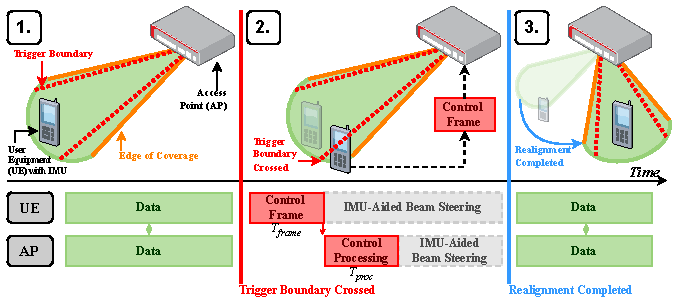
\includegraphics[width=0.95\linewidth]{Figures/Fig1.pdf}
\vspace{-8 pt}
\caption{Overview of JIT proactive beam management. (1)~Steady-state operation with continuous RF and IMU monitoring. (2)~Upon crossing the trigger boundary, the UE transmits a control frame ($T_{\text{frame}}$) containing its kinematic state \emph{just before} exiting the Edge of Coverage; the AP processes it ($T_{\text{proc}}$) and both nodes initiate beam steering. (3)~Realignment completes and the data link is restored. The bottom timeline shows the UE and AP activity during the procedure.}

\label{fig_alignment_pdf}
\vspace{-5pt}
\end{figure}

Conventional millimeter-wave beam management strategies typically operate reactively, initiating recovery procedures only after signal degradation or link failure is detected\cite{Giordani2018ATO, Wang2022}. This approach is challenging in sub-THz networks due to the reliance on high-gain antennas\cite{Kleine-Ostmann2011}. While essential for closing the link budget, narrow beams (with half-power beamwidths, HPBW, on the order of a few degrees) create mobility constraints: they quadratically expand the spatial search space while shrinking the beam residence time (the window where a moving node stays aligned).

The proposed JIT hybrid proactive+reactive sub-THz beam realignment approach, illustrated in Fig.~\ref{fig_alignment_pdf}, bridges this gap by leveraging IMU sensor data on a mobile UE to provide the access point (AP) with real-time motion awareness. The algorithm fuses RF and IMU data to continuously monitor the UE's deviation from the beam center. A trigger boundary, set inside the antenna's Edge of Coverage (EoC), determines when preemptive action is required. When the projected deviation crosses this boundary, the UE transmits a compact control frame containing its kinematic state to the AP before the link is lost. Then, both nodes initiate coordinated IMU-aided beam steering, completing realignment, or, when prevention is not possible, facilitating a deterministic prompt recovery. Additionally, JIT leverages the sub-THz spectrum to transmit control frames with microsecond-level latency, allowing the system to react to mobility events within the short beam residence time.

To validate this proposal, we implemented the JIT solution using the MobileTHz platform, encompassing both a high-fidelity software simulator and a hardware platform (detailed in the \textit{Methods} section). We then performed a comparative study, benchmarking the performance of the JIT beam realignment against two conventional reactive approaches: the Hierarchical Search algorithm and the IMU-Assist algorithm. The details of the study, including experimental assumptions and system parameters, are summarized in \textit{Methods}, while the key results of our evaluation are discussed in the \textit{Results} section.



%-------------------------------------------------------------------%
%-------------------------------------------------------------------%
%-------------------------------------------------------------------%
\section*{Results}

\rev{\subsection*{Experimental Setup and Performance Metrics}}

We benchmark JIT against four reference schemes. The first two are: (i)~a \rev{state-of-the-art Hierarchical Search beam recovery approach (without IMU assistance)\cite{photonics11060540}, consistent with the SSB-based beam search defined for 3GPP NR\cite{Giordani2018ATO, Heng2021SixChallenges}}; and (ii)~a reactive IMU-assisted beam alignment (leveraging IMU data for beam realignment, but without JIT signaling)\rev{\cite{s141019622, Brambilla_2019, 9391649}}. For illustration, we also model (iii)~a pure static (no realignment) baseline approach used in stationary sub-THz communication systems; and (iv)~a perfect alignment setup (a non-constructive Oracle-based optimal setup with continuous perfect beam alignment and no signaling overheads regardless of the nodes' mobility). The latter also serves as a theoretical upper bound for any constructive beam realignment approach.

\rev{We evaluate each scheme across four key performance indicators (KPIs), formally derived in the \textit{Evaluation Metrics} subsection of \textit{Methods}: \emph{Mean Capacity} ($\bar{C}$), the time-averaged Shannon capacity over the scenario duration; \emph{Capacity Coefficient of Variation (CoV)}, the normalized standard deviation of instantaneous capacity, capturing temporal stability; \emph{Link Availability} ($A_{\text{link}}$), the fraction of time the SNR meets or exceeds the 64-QAM threshold; and \emph{Signaling Overhead} ($O_{\text{sig}}$), the channel capacity foregone by JIT control-frame transmissions as a percentage of the total link capacity. Each group of results below sweeps a different input parameter: separation distance, UE translational acceleration, UE rotational acceleration, antenna directivity, and steering hardware constraints.}

\rev{For the steering hardware, we evaluate three representative models spanning practical sub-THz options (Table~\ref{tab:steering_and_hardware}): \textit{Constrained Mechanical} mirrors our laboratory testbed and anchors Hardware-in-the-Loop (HIL) validation; \textit{Ideal Mechanical} represents the upper bound of mechanical actuation for backhaul and UAV-style high-speed platforms; and \textit{Electronic} represents phased arrays envisioned for future mobile sub-THz access.}



%------------------------------------------------------------------%
\subsection*{Effects of Translational Acceleration on Beam Alignment}

We consider an AP and UE initially separated by $D_{initial} = 3$~m, an indoor short-range link\cite{9013236}. After a brief stationary period, the UE moves $D_{traversed} = 1.5$~m in a random direction relative to the AP, modeling human-scale mobility, such as walking between workstations. A representative received power profile for this scenario is shown in Fig.~\ref{fig:trans_metrics_example}.

\begin{figure}[ht!]
    \centering
        \begin{subfigure}{0.3275\linewidth}
        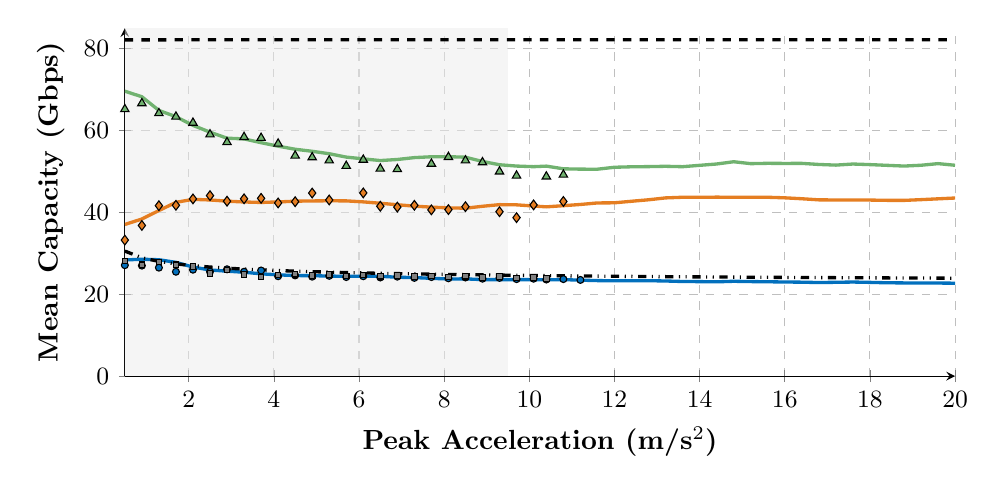
\begin{tikzpicture}
    \begin{axis}[
        width=\linewidth, height=6cm,
        xlabel={Peak Acceleration (m/s$^2$)},
        ylabel={Mean Capacity (Gbps)},
        legend style={
            font=\small,
            legend columns=2,
            legend pos=north east,
            inner sep=1pt,
            row sep=0pt,
            column sep=1pt,
            yshift=1pt,
            xshift=5pt
        },
        ymin=0,
        ymax=85
    ]
            \pgfplotsextra{
            \fill[gray!15, opacity=0.5] (axis cs:0, \pgfkeysvalueof{/pgfplots/ymin}) rectangle (axis cs:9.5, \pgfkeysvalueof{/pgfplots/ymax});
        }
        \addplot+[color=cb_blue, mark=none, solid, very thick]
            coordinates {
                (0.5, 28.37764120) (0.9, 28.55748432) (1.3, 28.43241005) (1.7, 27.78851984) (2.1, 26.63924368) (2.5, 25.93211920) (2.9, 25.63628528) (3.3, 25.38126315) (3.7, 24.99256793) (4.1, 24.73709173) (4.5, 24.57106482) (4.9, 24.53149721) (5.3, 24.44496426) (5.7, 24.37566188) (6.1, 24.38458396) (6.5, 24.38682203) (6.9, 24.15463529) (7.3, 24.07706384) (7.7, 23.88756521) (8.1, 23.72862681) (8.5, 23.75726537) (8.9, 23.57759309) (9.3, 23.58033259) (9.7, 23.57089460) (10.1, 23.56725765) (10.4, 23.54744846) (10.8, 23.57519162) (11.2, 23.44248456) (11.6, 23.33563752) (12.0, 23.28410217) (12.4, 23.29375588) (12.8, 23.31266206) (13.2, 23.23944793) (13.6, 23.11683496) (14.0, 23.08489350) (14.4, 23.03629103) (14.8, 23.16758994) (15.2, 23.09647703) (15.6, 23.05074031) (16.0, 22.99159486) (16.4, 22.94993782) (16.8, 22.85947364) (17.2, 22.92111636) (17.6, 22.98306822) (18.0, 22.89952905) (18.4, 22.80664974) (18.8, 22.76815973) (19.2, 22.74821630) (19.6, 22.73607044) (20.0, 22.69954647)
            };
        \addlegendentry{Blind Search (Sim.)}

        \addplot+[color=cb_orange, mark=none, solid, very thick]
            coordinates {
                (0.5, 37.04986331) (0.9, 38.38077769) (1.3, 40.45486988) (1.7, 42.45672274) (2.1, 43.18759033) (2.5, 43.03726310) (2.9, 42.74439476) (3.3, 42.54429082) (3.7, 42.43144846) (4.1, 42.55858511) (4.5, 42.73533196) (4.9, 42.80066503) (5.3, 42.83518138) (5.7, 42.81284652) (6.1, 42.56937616) (6.5, 42.23231238) (6.9, 41.86757325) (7.3, 41.52988753) (7.7, 41.28180198) (8.1, 41.10541461) (8.5, 41.02352265) (8.9, 41.49279035) (9.3, 41.89300138) (9.7, 41.84547669) (10.1, 41.55741949) (10.4, 41.35683119) (10.8, 41.63981467) (11.2, 41.93697785) (11.6, 42.30887998) (12.0, 42.34300888) (12.4, 42.71934429) (12.8, 43.08364638) (13.2, 43.54181880) (13.6, 43.69824678) (14.0, 43.69779342) (14.4, 43.72496590) (14.8, 43.70780256) (15.2, 43.70368694) (15.6, 43.69591042) (16.0, 43.55970447) (16.4, 43.33571410) (16.8, 43.06514798) (17.2, 43.03700703) (17.6, 43.03771275) (18.0, 43.01164476) (18.4, 42.94480378) (18.8, 42.93125012) (19.2, 43.11520631) (19.6, 43.31583937) (20.0, 43.51396864)
            };
        \addlegendentry{IMU-Assist (Sim.)}

        \addplot+[color=cb_green, mark=none, solid, very thick]
            coordinates {
                (0.5, 69.62115046) (0.9, 68.25164199) (1.3, 64.90744996) (1.7, 63.38839919) (2.1, 61.26378016) (2.5, 59.60043292) (2.9, 58.13213521) (3.3, 57.95854993) (3.7, 57.02877406) (4.1, 56.17993381) (4.5, 55.42846290) (4.9, 54.93096160) (5.3, 54.33455236) (5.7, 53.51099203) (6.1, 53.07703314) (6.5, 52.66641219) (6.9, 52.92792178) (7.3, 53.38704100) (7.7, 53.59270040) (8.1, 53.61311502) (8.5, 53.48411901) (8.9, 52.44590582) (9.3, 51.64266507) (9.7, 51.32039378) (10.1, 51.16986384) (10.4, 51.30447318) (10.8, 50.64999814) (11.2, 50.56701053) (11.6, 50.55606726) (12.0, 51.02640410) (12.4, 51.14347500) (12.8, 51.18626848) (13.2, 51.26236611) (13.6, 51.16695898) (14.0, 51.49848044) (14.4, 51.82478913) (14.8, 52.37680821) (15.2, 51.90783531) (15.6, 51.99173959) (16.0, 51.96313979) (16.4, 51.97812606) (16.8, 51.71382171) (17.2, 51.55308107) (17.6, 51.81767863) (18.0, 51.67441995) (18.4, 51.49996544) (18.8, 51.32111499) (19.2, 51.51804000) (19.6, 51.91619423) (20.0, 51.51484611)
            };
        \addlegendentry{JIT (Sim.)}

        \addplot+[color=black, mark=none, dashdotdotted, very thick]
            coordinates {
                (0.5, 30.543448308728504) (0.9, 28.92094695925334) (1.3, 28.02129644490966) (1.7, 27.423160073632452) (2.1, 26.98640348973689) (2.5, 26.646911425187646) (2.9, 26.3738272876669) (3.3, 26.14732197248137) (3.7, 25.955464578924953) (4.1, 25.789940890165063) (4.5, 25.644951703837627) (4.9, 25.51669113702047) (5.3, 25.402441420747337) (5.7, 25.299747621985475) (6.1, 25.2063440644451) (6.5, 25.120820754189353) (6.9, 25.04249705164348) (7.3, 24.970289301661786) (7.7, 24.903563526352674) (8.1, 24.84135776717663) (8.5, 24.783555836188086) (8.9, 24.729216421826646) (9.3, 24.67836243679004) (9.7, 24.630654018124023) (10.1, 24.585546359760137) (10.4, 24.5429605931815) (10.8, 24.502628369576524) (11.2, 24.46423229512446) (11.6, 24.42760181911845) (12.0, 24.392750975594435) (12.4, 24.359834291265948) (12.8, 24.328356637318414) (13.2, 24.297958893818617) (13.6, 24.268844277150937) (14.0, 24.240822909091538) (14.4, 24.214035829156824) (14.8, 24.18829635748286) (15.2, 24.16344837167031) (15.6, 24.139636657644886) (16.0, 24.11676910702295) (16.4, 24.094614790922535) (16.8, 24.073257411167038) (17.2, 24.05241218453326) (17.6, 24.032414476460012) (18.0, 24.01296909571691) (18.4, 23.994167831933215) (18.8, 23.975951284712405) (19.2, 23.95832028968138) (19.6, 23.941325690921403) (20.0, 23.924646069277216)
            };
        \addlegendentry{Static (Sim.)}
                
        \addplot+[color=black, mark=none, dashed, very thick]
            coordinates {
                (0.5, 82.14747650644048) (0.9, 82.15517869739426) (1.3, 82.15944742352464) (1.7, 82.16228991048158) (2.1, 82.16436865536933) (2.5, 82.16597479660588) (2.9, 82.16727049697342) (3.3, 82.16834444625654) (3.7, 82.16925550381866) (4.1, 82.1700409822356) (4.5, 82.17072672500095) (4.9, 82.171332903018) (5.3, 82.17187575591124) (5.7, 82.17236523783842) (6.1, 82.17280792686356) (6.5, 82.17321125245627) (6.9, 82.17358197595405) (7.3, 82.17392371105402) (7.7, 82.17424069415235) (8.1, 82.17453457758761) (8.5, 82.17480988263529) (8.9, 82.17506632362236) (9.3, 82.17530788846815) (9.7, 82.17553583732987) (10.1, 82.17575036212091) (10.4, 82.17595351690429) (10.8, 82.17614591648935) (11.2, 82.17632828040549) (11.6, 82.17650109750709) (12.0, 82.17666590439323) (12.4, 82.17682458270806) (12.8, 82.1769759546025) (13.2, 82.17711964540845) (13.6, 82.17725754139956) (14.0, 82.17738926348122) (14.4, 82.17751637109045) (14.8, 82.17763857768612) (15.2, 82.17775590837445) (15.6, 82.17786945130857) (16.0, 82.17797907886663) (16.4, 82.17808485241152) (16.8, 82.17818691425079) (17.2, 82.17828500299878) (17.6, 82.17838027111054) (18.0, 82.1784722693721) (18.4, 82.17856159608786) (18.8, 82.17864825980098) (19.2, 82.17873252116941) (19.6, 82.17881462006233) (20.0, 82.17889363129288)
            };
        \addlegendentry{Theoretical Max}
        
        \addplot+[
            color=black, 
            only marks,
            mark=*,
            mark size=1.25pt,
            mark options={fill=cb_blue, solid} 
        ]
            coordinates {
                (0.5, 27.1) (0.9, 27.0) (1.3, 26.5) (1.7, 25.5) (2.1, 26.0) (2.5, 25.5) (2.9, 26.1) (3.3, 25.5) (3.7, 25.8) (4.1, 24.4) (4.5, 24.6) (4.9, 24.3) (5.3, 24.5) (5.7, 24.2) (6.1, 24.4) (6.5, 24.1) (6.9, 24.3) (7.3, 24.0) (7.7, 24.2) (8.1, 23.9) (8.5, 24.1) (8.9, 23.8) (9.3, 24.0) (9.7, 23.7) (10.1, 23.8) (10.4, 23.6) (10.8, 23.7) (11.2, 23.5)
            };
        \addlegendentry{Blind Search (Exp.)}

        \addplot+[
            color=black, 
            only marks,
            mark=square*,
            mark size=1pt,
            mark options={fill=gray, solid}
        ]
            coordinates {
                (0.5, 28.1) (0.9, 27.2) (1.3, 27.9) (1.7, 27.2) (2.1, 26.8) (2.5, 25.1) (2.9, 25.9) (3.3, 24.8) (3.7, 24.2) (4.1, 24.7) (4.5, 24.9) (4.9, 24.6) (5.3, 24.8) (5.7, 24.5) (6.1, 24.7) (6.5, 24.4) (6.9, 24.6) (7.3, 24.3) (7.7, 24.5) (8.1, 24.2) (8.5, 24.4) (8.9, 24.1) (9.3, 24.3) (9.7, 24.0) (10.1, 24.1) (10.4, 23.9)
            };
        \addlegendentry{Static (Exp.)}

        \addplot+[
            color=black, 
            only marks,
            mark=diamond*,
            mark size=1.75pt,
            mark options={fill=cb_orange, solid}
        ]
            coordinates {
                (0.5, 33.23746891) (0.9, 36.81073287) (1.3, 41.64006548) (1.7, 41.73750084) (2.1, 43.29048249) (2.5, 44.09074373) (2.9, 42.73490841) (3.3, 43.32530586) (3.7, 43.44130010) (4.1, 42.30319201) (4.5, 42.61182364) (4.9, 44.72732400) (5.3, 43.03421619) (6.1, 44.75921784) (6.5, 41.50010486) (6.9, 41.29289080) (7.3, 41.73745904) (7.7, 40.61919706) (8.1, 40.68006087) (8.5, 41.39289688) (9.3, 40.16727644) (9.7, 38.71377820) (10.1, 41.83013474) (10.8, 42.66772779)
            };
        \addlegendentry{IMU-Assist (Sim.)}

        \addplot+[
            color=black, 
            only marks,
            mark=triangle*,
            mark size=1.75pt,
            mark options={fill=cb_green, solid}
        ]
            coordinates {
                (0.5, 65.20533604) (0.9, 66.65919385) (1.3, 64.22106079) (1.7, 63.38534701) (2.1, 61.89129385) (2.5, 59.03716576) (2.9, 57.13380661) (3.3, 58.40434661) (3.7, 58.18669856) (4.1, 56.79381030) (4.5, 53.86034281) (4.9, 53.44761186) (5.3, 52.67757716) (5.7, 51.34474727) (6.1, 52.85246066) (6.5, 50.68149553) (6.9, 50.54583959) (7.7, 51.87841316) (8.1, 53.51853016) (8.5, 52.68906212) (8.9, 52.22916259) (9.3, 49.97418795) (9.7, 48.97295284) (10.4, 48.76320670) (10.8, 49.20009688)
            };
        \addlegendentry{JIT (Sim.)}

        \legend{}
    \end{axis}
\end{tikzpicture}
        \vspace{-25pt}
        \caption{Constrained Mechanical Steering}
        \label{fig:trans_exp_rate}
    \end{subfigure}
    \hfill
    \begin{subfigure}{0.3275\linewidth}
    \include{Figures/Fig2b}
        \vspace{-25pt}
        \caption{Ideal Mechanical Steering}
        \label{fig:trans_sim_rate}
    \end{subfigure}
    \hfill
    \begin{subfigure}{0.3275\linewidth}
        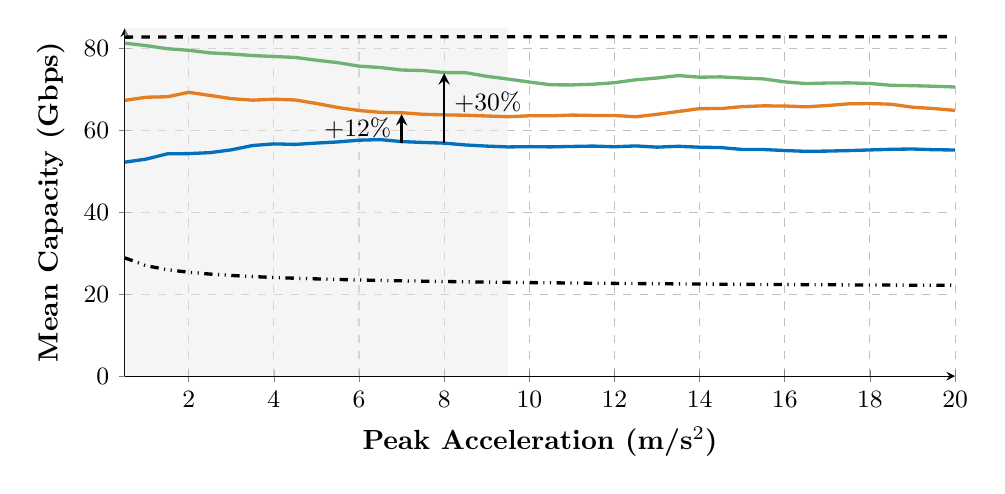
\begin{tikzpicture}
    \begin{axis}[
        width=\linewidth, height=6cm,
        xlabel={Peak Acceleration (m/s$^2$)},
        ylabel={Mean Capacity (Gbps)},
        ymin=0,
        ymax=85
    ]
                \pgfplotsextra{
            \fill[gray!15, opacity=0.5] (axis cs:0, \pgfkeysvalueof{/pgfplots/ymin}) rectangle (axis cs:9.5, \pgfkeysvalueof{/pgfplots/ymax});
        }
        \addplot+[color=cb_blue, mark=none, solid, very thick]
            coordinates {
                (0.5, 52.27783985)
                (1.0, 53.01944841)
                (1.5, 54.31676328)
                (2.0, 54.36138690)
                (2.5, 54.59890697)
                (3.0, 55.28328015)
                (3.5, 56.33999059)
                (4.0, 56.73681331)
                (4.5, 56.61214636)
                (5.0, 56.94067898)
                (5.5, 57.21575017)
                (6.0, 57.64430428)
                (6.5, 57.78676454)
                (7.0, 57.29575364)
                (7.5, 57.09329337)
                (8.0, 56.92166814)
                (8.5, 56.47700542)
                (9.0, 56.19708876)
                (9.5, 55.99420983)
                (10.0, 56.06562113)
                (10.5, 56.00760971)
                (11.0, 56.11343356)
                (11.5, 56.20206718)
                (12.0, 56.04081600)
                (12.5, 56.24084814)
                (13.0, 55.94504801)
                (13.5, 56.14849006)
                (14.0, 55.93367739)
                (14.5, 55.83448046)
                (15.0, 55.37633530)
                (15.5, 55.36091835)
                (16.0, 55.11704630)
                (16.5, 54.91455068)
                (17.0, 54.97970442)
                (17.5, 55.09752592)
                (18.0, 55.26096279)
                (18.5, 55.41666656)
                (19.0, 55.49017902)
                (19.5, 55.31150792)
                (20.0, 55.24905353)
            };
        \addlegendentry{Baseline}
        \addplot+[color=cb_orange, mark=none, solid, very thick]
            coordinates {
                (0.5, 67.37650771)
                (1.0, 68.13780049)
                (1.5, 68.26073502)
                (2.0, 69.33074461)
                (2.5, 68.57735677)
                (3.0, 67.79620280)
                (3.5, 67.42370385)
                (4.0, 67.65392078)
                (4.5, 67.46799509)
                (5.0, 66.61961613)
                (5.5, 65.63569167)
                (6.0, 64.89746613)
                (6.5, 64.44630204)
                (7.0, 64.35218749)
                (7.5, 63.96927620)
                (8.0, 63.82922122)
                (8.5, 63.73690704)
                (9.0, 63.55252288)
                (9.5, 63.37875397)
                (10.0, 63.60400774)
                (10.5, 63.59622947)
                (11.0, 63.77799172)
                (11.5, 63.69071183)
                (12.0, 63.67242451)
                (12.5, 63.36475130)
                (13.0, 63.96312384)
                (13.5, 64.65470501)
                (14.0, 65.35205582)
                (14.5, 65.37559573)
                (15.0, 65.84881852)
                (15.5, 66.03058543)
                (16.0, 65.99533887)
                (16.5, 65.79826913)
                (17.0, 66.10913884)
                (17.5, 66.52565227)
                (18.0, 66.60899732)
                (18.5, 66.42705287)
                (19.0, 65.70030548)
                (19.5, 65.37240102)
                (20.0, 64.91791201)
            };
        \addlegendentry{IMU-Assist}
        \addplot+[color=cb_green, mark=none, solid, very thick]
            coordinates {
                (0.5, 81.34318220)
                (1.0, 80.74689379)
                (1.5, 79.99032581)
                (2.0, 79.61315763)
                (2.5, 78.97418004)
                (3.0, 78.70602349)
                (3.5, 78.32060299)
                (4.0, 78.09169671)
                (4.5, 77.86403374)
                (5.0, 77.18816358)
                (5.5, 76.58964893)
                (6.0, 75.73828468)
                (6.5, 75.40348982)
                (7.0, 74.78397397)
                (7.5, 74.66938173)
                (8.0, 74.16194886)
                (8.5, 74.14369573)
                (9.0, 73.25408534)
                (9.5, 72.57771447)
                (10.0, 71.85364887)
                (10.5, 71.17865536)
                (11.0, 71.14632813)
                (11.5, 71.32735639)
                (12.0, 71.68698286)
                (12.5, 72.40038916)
                (13.0, 72.83135592)
                (13.5, 73.42719540)
                (14.0, 73.03169917)
                (14.5, 73.11535245)
                (15.0, 72.83394176)
                (15.5, 72.61279446)
                (16.0, 71.88535818)
                (16.5, 71.47733163)
                (17.0, 71.60706249)
                (17.5, 71.64824173)
                (18.0, 71.49451936)
                (18.5, 71.04325096)
                (19.0, 70.96391979)
                (19.5, 70.82033794)
                (20.0, 70.63881928)
            };
        \addlegendentry{JIT}
        \addplot+[color=black, mark=none, dashdotdotted, very thick]
            coordinates {
                (0.5, 28.8947382101455)
                (1.0, 26.969169115927166)
                (1.5, 25.995251264918235)
                (2.0, 25.374237404533286)
                (2.5, 24.92926446632614)
                (3.0, 24.590751629669978)
                (3.5, 24.32109460968743)
                (4.0, 24.099123634295022)
                (4.5, 23.912374514076923)
                (5.0, 23.752233453377162)
                (5.5, 23.613186329384398)
                (6.0, 23.49032548990613)
                (6.5, 23.380750314732047)
                (7.0, 23.28247705286013)
                (7.5, 23.193600790438502)
                (8.0, 23.112763873161796)
                (8.5, 23.038622108812728)
                (9.0, 22.970434039097313)
                (9.5, 22.907447300678758)
                (10.0, 22.849093680864257)
                (10.5, 22.79485329391962)
                (11.0, 22.74408617922097)
                (11.5, 22.696273456515772)
                (12.0, 22.65120415882518)
                (12.5, 22.6092946082088)
                (13.0, 22.569441313879537)
                (13.5, 22.531621325766363)
                (14.0, 22.495463237143365)
                (14.5, 22.461407151520792)
                (15.0, 22.428869495834956)
                (15.5, 22.39781355099796)
                (16.0, 22.368538474922936)
                (16.5, 22.340311733826315)
                (17.0, 22.31335184738684)
                (17.5, 22.28736949694756)
                (18.0, 22.26243919670142)
                (18.5, 22.238548886575717)
                (19.0, 22.215543563218016)
                (19.5, 22.19358536685704)
                (20.0, 22.17229811981071)
            };
        \addlegendentry{No Alignment (Static)}
        \addplot+[color=cb_black, mark=none, dashed, very thick]
            coordinates {
                (0.5, 82.82446846555551)
                (1.0, 82.8571849762413)
                (1.5, 82.87373338773737)
                (2.0, 82.88430563834424)
                (2.5, 82.89184527283311)
                (3.0, 82.8975950543959)
                (3.5, 82.90217414469629)
                (4.0, 82.90593820389594)
                (4.5, 82.90910738410987)
                (5.0, 82.91182464406593)
                (5.5, 82.9141911320053)
                (6.0, 82.91627516636049)
                (6.5, 82.91813057437744)
                (7.0, 82.9197966373228)
                (7.5, 82.92130430608232)
                (8.0, 82.92267698778764)
                (8.5, 82.92393411110231)
                (9.0, 82.92509124331261)
                (9.5, 82.9261613589891)
                (10.0, 82.927155403492)
                (10.5, 82.92808126301999)
                (11.0, 82.92894685993251)
                (11.5, 82.92975783575129)
                (12.0, 82.93051950835635)
                (12.5, 82.93123912303135)
                (13.0, 82.93191863271645)
                (13.5, 82.93256081209971)
                (14.0, 82.93316976345672)
                (14.5, 82.9337486383414)
                (15.0, 82.93429971838061)
                (15.5, 82.93482526779735)
                (16.0, 82.93532806868741)
                (16.5, 82.93580866007558)
                (17.0, 82.93626835072722)
                (17.5, 82.9367088127152)
                (18.0, 82.9371316550052)
                (18.5, 82.93753829261286)
                (19.0, 82.93792906738264)
                (19.5, 82.9383059676947)
                (20.0, 82.93866881601643)
            };
        \addlegendentry{Theoretical Max}
        \legend{}

        \draw[<-, >=stealth, thick] (axis cs:8, 74) -- (axis cs:8, 57)
             node[midway, right=0pt, font=\small, yshift=2pt] {$+30\%$};

         \draw[<-, >=stealth, thick] (axis cs:7, 64) -- (axis cs:7, 57)
             node[midway, left=0pt, font=\small] {$+12\%$};
    \end{axis}
\end{tikzpicture}
        \vspace{-25pt}
        \caption{Electronic Steering}
        \label{fig:trans_simfast_rate}
    \end{subfigure}

    \vspace{8 pt}

    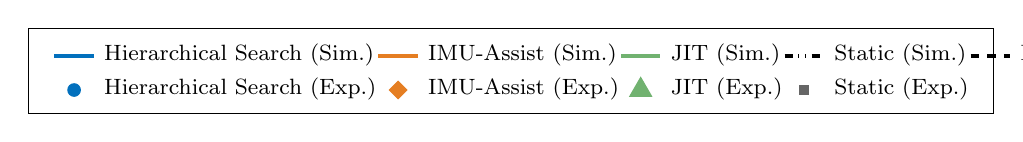
\begin{tikzpicture}
        \node [
            draw=black,
            line width=0.5pt,
            inner sep=3pt,
            rounded corners=0pt,
            align=center
        ] {
            \footnotesize
            \setlength{\tabcolsep}{0pt}
            \renewcommand{\arraystretch}{1.3} % Vertical spacing between Sim and Exp rows

            \begin{tabular*}{\dimexpr0.969\linewidth}{
                c @{\extracolsep{0pt}\hspace{3pt}} l
                @{\extracolsep{\fill}}
                c @{\extracolsep{0pt}\hspace{3pt}} l
                @{\extracolsep{\fill}}
                c @{\extracolsep{0pt}\hspace{3pt}} l
                @{\extracolsep{\fill}}
                c @{\extracolsep{0pt}\hspace{3pt}} l
                @{\extracolsep{\fill}}
                c @{\extracolsep{0pt}\hspace{3pt}} l
            }

                % --- ROW 1: SIMULATIONS ---
                \legline{cb_blue}{solid} & Hierarchical Search (Sim.) &
                \legline{cb_orange}{solid} & IMU-Assist (Sim.) &
                \legline{cb_green}{solid} & JIT (Sim.) &
                \legline{black}{dashdotdotted} & Static (Sim.) &
                \legline{black}{dashed} & Perfect Alignment (Sim.) \\

                % --- ROW 2: EXPERIMENTS ---
                \legmark{cb_blue}{circle} & Hierarchical Search (Exp.) &
                \legmark{cb_orange}{diamond} & IMU-Assist (Exp.) &
                \legmark{cb_green}{regular polygon, regular polygon sides=3} & JIT (Exp.) &
                \legmark{cb_dark_gray}{rectangle} & Static (Exp.) &
                 & % Empty cell under Perfect Alignment

            \end{tabular*}
        };
    \end{tikzpicture}

    \caption{Translational mobility evaluation ($D_{initial} = 3$~m, $D_{traversed} = 1.5$~m) across three steering models. HIL markers in~(a) validate simulation with MAPE of 1.80--3.13\% and NRMSE of 2.99--3.82\%. Percentage annotations in~(b,\,c) are relative to Hierarchical Search at the marked acceleration.}
    \label{fig:translational_rate}
    \vspace{-5pt}
\end{figure}

Under the Constrained Mechanical model (Fig.~\ref{fig:trans_exp_rate}), slow mechanical steering imposes the harshest penalty on every realignment attempt. Under these constraints, Hierarchical Search frequently fails to complete its scan before the UE moves away, causing it to achieve 5–7\% worse mean capacity than a static, non-steered link across the acceleration range. The IMU-Assist algorithm mitigates this by narrowing the angular search space using on-device motion estimates, improving mean capacity over Hierarchical Search by up to 92\% at \SI{20}{m/s^2}. JIT further extends this advantage by preemptively sharing kinematics with the AP, achieving up to an 88\% improvement over IMU-Assist at low accelerations. At the highest mobility, IMU-Assist and JIT reach 50\% and 69\% of the theoretical maximum, respectively, confirming that sensor-informed algorithms can make mechanically constrained hardware viable for mobile links where a purely reactive approach cannot.

To validate these simulation results, we conducted Hardware-in-the-Loop experiments across all four algorithm configurations. The experimental data closely matched the simulation, with Mean Absolute Percentage Error (MAPE) values of 1.80--3.13\% and Normalized Root Mean Square Error (NRMSE) of 2.99--3.82\%, confirming that the MobileTHz engine captures the physical constraints of the steering hardware. The subsequent analysis therefore uses simulation to explore steering models beyond our laboratory equipment.

Under the Ideal Mechanical model (Fig.~\ref{fig:trans_sim_rate}), faster rotary movements impose a lower opportunity cost than the Constrained Mechanical model. Hierarchical Search now outperforms the static reference by at least 75\%, since the faster hardware can complete enough scan iterations within the beam residence time to recover alignment. IMU-Assist provides further gains of up to 39\% at \SI{20}{m/s^2}, though it slightly underperforms at \SI{0.5}{m/s^2} due to overshooting from aggressive motion prediction (discussed in Methods). JIT delivers the largest improvement across the full range, narrowing the gap to the theoretical maximum by synchronizing both nodes rather than relying on the AP's reactive scan alone. This result demonstrates that even when hardware is fast enough for reactive recovery to succeed, proactive coordination still yields additional gains by eliminating unnecessary search overhead.

With the Electronic model (Fig.~\ref{fig:trans_simfast_rate}), where steering latency is negligible, the performance spread narrows: Hierarchical Search plateaus at \SI{55.3}{Gbps}, IMU-Assist at \SI{63.4}{Gbps}, and JIT at \SI{72.6}{Gbps}. Yet JIT still retains a 12\% advantage over IMU-Assist and 30\% over Hierarchical Search, showing that the search-space penalty of reactive methods persists even when hardware is no longer the bottleneck.

\begin{figure*}[ht!]
    \centering
    \begin{subfigure}[t]{0.475\textwidth}
        \vspace{0pt}
        \centering
        \input{Figures/Fig3a}
        \vspace{-20pt}
        \caption{Captured Rx Power across entire movement scenario}
        \label{fig:trans_metrics_example}
    \end{subfigure}%
    \hfill
    \begin{minipage}[t]{0.475\textwidth}
        \vspace{0pt}
        \centering
        \begin{subfigure}{\linewidth}
            \input{Figures/Fig3b}
            \vspace{-15pt}
            \caption{Capacity Coefficient of Variation}
            \label{fig:trans_metrics_covariance}
        \end{subfigure}
        \vfill
            \begin{subfigure}{\linewidth}
            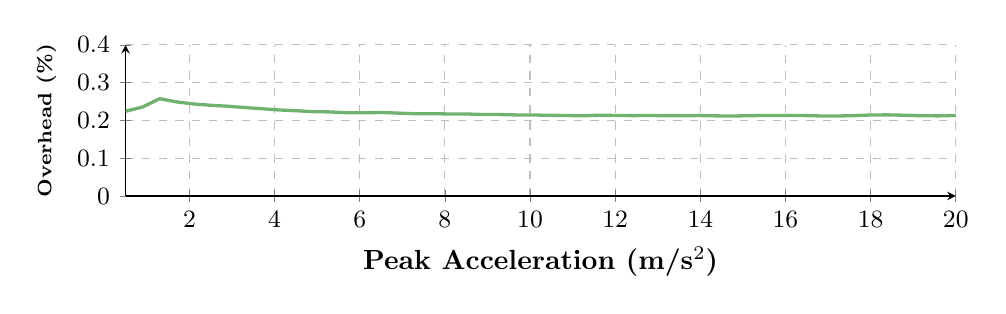
\begin{tikzpicture}
    \begin{axis}[
        width=\linewidth, height=3.5cm,
        xlabel={Peak Acceleration (m/s$^2$)},
        ylabel={Overhead (\%)},
        ylabel style={
            font=\scriptsize\bfseries,
            align=center 
        },
        ymin=0,
        ymax=0.4,
        yticklabel style={
            text width=1.25em,
            align=right,
        },
    ]
        \addplot+[color=cb_green, mark=none, solid, very thick]
            coordinates {
                (0.5, 0.22420112)
                (0.9, 0.23569438)
                (1.3, 0.25754338)
                (1.7, 0.24909822)
                (2.1, 0.24358554)
                (2.5, 0.24016843)
                (2.9, 0.23767637)
                (3.3, 0.23416817)
                (3.7, 0.23111576)
                (4.1, 0.22780320)
                (4.5, 0.22577956)
                (4.9, 0.22326105)
                (5.3, 0.22258990)
                (5.7, 0.22038953)
                (6.1, 0.22024583)
                (6.5, 0.22115591)
                (6.9, 0.21942761)
                (7.3, 0.21781039)
                (7.7, 0.21794326)
                (8.1, 0.21708757)
                (8.5, 0.21720379)
                (8.9, 0.21563414)
                (9.3, 0.21567145)
                (9.7, 0.21451458)
                (10.1, 0.21452723)
                (10.4, 0.21355301)
                (10.8, 0.21325653)
                (11.2, 0.21240689)
                (11.6, 0.21358425)
                (12.0, 0.21330081)
                (12.4, 0.21281653)
                (12.8, 0.21300542)
                (13.2, 0.21272336)
                (13.6, 0.21266974)
                (14.0, 0.21295267)
                (14.4, 0.21205256)
                (14.8, 0.21179770)
                (15.2, 0.21273656)
                (15.6, 0.21331308)
                (16.0, 0.21327360)
                (16.4, 0.21310839)
                (16.8, 0.21198160)
                (17.2, 0.21174075)
                (17.6, 0.21266866)
                (18.0, 0.21450954)
                (18.4, 0.21473516)
                (18.8, 0.21379288)
                (19.2, 0.21253728)
                (19.6, 0.21210702)
                (20.0, 0.21325361)
            };
        \addlegendentry{JIT}
        \legend{}
    \end{axis}
\end{tikzpicture}
            \vspace{-15pt}
            \caption{Signaling Overhead}
            \label{fig:trans_metrics_overhead}
        \end{subfigure}
    \end{minipage}
    \caption{Ideal Mechanical, translational scenario ($D_{initial} = 3$~m, $D_{traversed} = 1.5$~m, $3.0$~m/s$^2$ peak). (a)~Single-run trace at $3.0$~m/s$^2$; shaded region indicates UE displacement interval. (b,\,c)~Aggregated over the full acceleration sweep.}
    \label{fig:translational_metrics}
    \vspace{-5pt}
\end{figure*}

Although mean capacity summarizes maximum link performance, it masks temporal variance, making it insufficient as a sole metric for assessing mobile link robustness. A single mobility event is illustrated in Fig.~\ref{fig:trans_metrics_example}, showcasing the power variations over time. Hierarchical Search experiences the most power oscillations during movement, while the IMU-Assist algorithm decreases temporal variance as well as the magnitude of link loss. JIT outperforms the other algorithms, providing a stable link and the highest final received power of \SI{-12.7}{dBm}.

The CoV of the capacity across the three algorithms is quantified in Fig.~\ref{fig:trans_metrics_covariance} as peak acceleration increases under the Ideal Mechanical model. The IMU-Assist algorithm reduces CoV by up to 66\% compared to Hierarchical Search, demonstrating that IMU integration improves not only mean capacity (as shown in Fig.~\ref{fig:trans_sim_rate}, where IMU-Assist achieved up to a 39\% increase) but also reduces capacity variance. However, single-node motion compensation alone is insufficient to achieve a consistently low-variance link. JIT shows that capacity variance can be further reduced when both nodes share mobility awareness, reducing CoV by up to 89.2\% compared to Hierarchical Search and by 23.7\% compared to IMU-Assist.

Overhead, defined as the potential channel capacity consumed by JIT transmission, is quantified in Fig.~\ref{fig:trans_metrics_overhead}. Overhead increases up to \SI{1.3}{m/s^2}, the point at which the UE consistently moves beyond the AP's EoC causing more realignment events. At higher accelerations, however, overhead decreases as the AP's look-ahead strategy results in fewer intermediate realignments before the UE reaches its final position. Overall, JIT improves mean capacity and reduces link variance while consuming at most 0.26\% of the total channel capacity, demonstrating its efficiency in high-mobility regimes.

\rev{A small residual gap between JIT and the Perfect Alignment reference is visible in the steady-state portion of Fig.~\ref{fig:trans_metrics_example}. By design, JIT does not continuously chase the maximum SNR; it triggers realignment only when the projected angular displacement is about to cross $\eta \cdot \theta_{\text{HPBW}} = 0.36 \cdot \SI{13}{\degree} \approx \SI{4.7}{\degree}$ (Eq.~\ref{eq:trigger}). Between triggers, the UE may sit slightly off-axis without correction, while the Perfect Alignment reference assumes zero misalignment at every instant.}



%-------------------------------------------------------------------%
\subsection*{Effects of Rotational Acceleration on Beam Alignment}

\begin{figure}[ht!]
    \centering
    \begin{subfigure}{0.3275\linewidth}
        \include{Figures/Fig4a}
        \vspace{-25pt}
        \caption{Constrained Mechanical Steering}
        \label{fig:rot_exp_rate}
    \end{subfigure}
    \hfill
    \begin{subfigure}{0.3275\linewidth}
        \include{Figures/Fig4b}
        \vspace{-25pt}
        \caption{Ideal Mechanical Steering}
        \label{fig:rot_sim_rate}
    \end{subfigure}
    \hfill
    \begin{subfigure}{0.3275\linewidth}
        \include{Figures/Fig4c}
        \vspace{-25pt}
        \caption{Electronic Steering}
        \label{fig:rot_simfast_rate}
    \end{subfigure}

    \vspace{5 pt}

    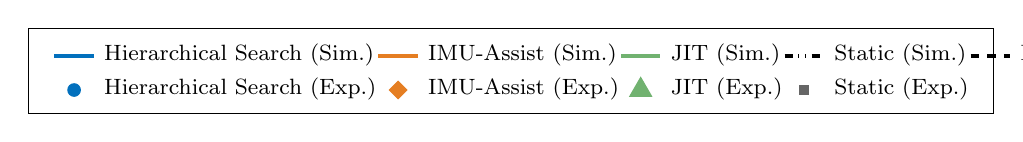
\begin{tikzpicture}
        \node [
            draw=black,
            line width=0.5pt,
            inner sep=3pt,
            rounded corners=0pt,
            align=center
        ] {
            \footnotesize
            \setlength{\tabcolsep}{0pt}
            \renewcommand{\arraystretch}{1.3} % Vertical spacing between Sim and Exp rows
            \begin{tabular*}{\dimexpr0.969\linewidth}{
                c @{\extracolsep{0pt}\hspace{3pt}} l
                @{\extracolsep{\fill}}
                c @{\extracolsep{0pt}\hspace{3pt}} l
                @{\extracolsep{\fill}}
                c @{\extracolsep{0pt}\hspace{3pt}} l
                @{\extracolsep{\fill}}
                c @{\extracolsep{0pt}\hspace{3pt}} l
                @{\extracolsep{\fill}}
                c @{\extracolsep{0pt}\hspace{3pt}} l
            }

                % --- ROW 1: SIMULATIONS ---
                \legline{cb_blue}{solid} & Hierarchical Search (Sim.) &
                \legline{cb_orange}{solid} & IMU-Assist (Sim.) &
                \legline{cb_green}{solid} & JIT (Sim.) &
                \legline{black}{dashdotdotted} & Static (Sim.) &
                \legline{black}{dashed} & Perfect Alignment (Sim.) \\

                % --- ROW 2: EXPERIMENTS ---
                \legmark{cb_blue}{circle} & Hierarchical Search (Exp.) &
                \legmark{cb_orange}{diamond} & IMU-Assist (Exp.) &
                \legmark{cb_green}{regular polygon, regular polygon sides=3} & JIT (Exp.) &
                \legmark{cb_dark_gray}{rectangle} & Static (Exp.) &
                 & % Empty cell under Perfect Alignment

            \end{tabular*}
        };
    \end{tikzpicture}
    \caption{Rotational mobility evaluation ($D_{initial} = 3$~m, $45^\circ$ displacement) across three steering models. Hierarchical Search falls below the static reference in all cases due to misdirected AP scanning. HIL validation in~(a): MAPE of 3.88--4.68\% for JIT and IMU-Assist; higher for Hierarchical Search (11.66\%) due to low absolute capacity.}
    \label{fig:rotational_rate}
    \vspace{-5pt}
\end{figure}

Rotational motion often presents the greatest challenge to beam management, as typical angular rates from rotation can be significantly higher than those induced by translation\cite{9391649} (see also Supplementary Figs.~1 and~2). Unlike translation, where the geometric Line-of-Sight (LoS) angle changes at both nodes and both must steer to compensate, pure rotation alters only the UE's orientation, and the AP's LoS remains unchanged. The correct response is therefore for the UE to counter-rotate while the AP holds its position. Reactive algorithms, relying solely on RF power drops, cannot distinguish rotation from translation and default to searching at both nodes. Under pure rotation, this causes the AP to actively steer \emph{away} from the correct direction, turning the recovery mechanism itself into a source of misalignment.

This behavior is quantified in Fig.~\ref{fig:rot_sim_rate}, where Hierarchical Search's capacity degrades to \SI{5}{}--\SI{6}{Gbps}, consistently falling below the static reference across the full acceleration range. The IMU-Assist algorithm addresses this failure at one node: the UE uses on-device sensor data to identify the motion as rotation and counter-rotates to maintain alignment rather than initiating a scan, recovering capacity to approximately \SI{30}{Gbps}. However, this correction is local to the UE. The AP, unaware that the UE has already compensated, may still detect a transient power drop and trigger its own reactive scan, partially undoing the UE's correction. This coordination gap caps IMU-Assist at around 36.5\% of the theoretical maximum. JIT closes this gap, sustaining capacity above \SI{55}{Gbps} up to \SI{120}{deg/s^2}. Even at \SI{300}{deg/s^2}, representative of the upper range of human rotational acceleration (see Supplementary Figs.~1 and~2), JIT maintains a 47\% advantage over IMU-Assist.

The Electronic model (Fig.~\ref{fig:rot_simfast_rate}) also demonstrates that Hierarchical Search remains below the static reference, since fast steering cannot correct a misdirected search. IMU-Assist recovers to approximately \rev{\SI{38}{Gbps}} at \rev{\SI{700}{deg/s^2}}, while JIT sustains above \SI{57}{Gbps} across the full range by ensuring the AP holds position rather than scanning.

Under experimental constraints (Fig.~\ref{fig:rot_exp_rate}), all algorithms degrade more rapidly than in the idealized scenarios because the rotary stages cannot complete the required angular correction within the beam residence time. Hierarchical Search remains at \SI{7}{}--\SI{8}{Gbps} throughout, consistently below the static reference. IMU-Assist falls from \SI{43}{Gbps} to under \SI{10}{Gbps} by \SI{100}{deg/s^2}, while JIT drops from \SI{60}{Gbps} to \SI{30}{Gbps} over the same interval, retaining a $3\times$ capacity advantage, demonstrating that hybrid proactive+reactive coordination can extend the usable rotational range of mechanically steered systems well beyond what reactive algorithms support. Experimental results track simulation with MAPE of 3.88--11.66\% and NRMSE of 5.19--17.5\%, with the higher errors concentrated in Hierarchical Search, where low absolute capacities amplify small deviations. JIT and IMU-Assist show closer agreement (MAPE of 3.88\% and 4.68\%), validating the MobileTHz engine under rotational dynamics.

While capacity CoV (Fig.~\ref{fig:trans_metrics_covariance}) quantifies variance over the entire scenario, it does not indicate what fraction of time the link actually sustains the data rates that sub-THz systems are designed to deliver\cite{Dang2020, Nokia2022}. Link availability addresses this by measuring the fraction of time SNR exceeds \SI{18.8}{dB} (derived in \textit{Evaluation Metrics} subsection). A system may exhibit low CoV yet poor link availability if it sustains a steady but weak signal below the modulation threshold.

\begin{figure}[h!]
    \centering
    \begin{subfigure}{0.495\linewidth}
        \include{Figures/Fig5a}
        \vspace{-25pt}
        \caption{Link Availability vs. Peak rotational acceleration}
        \label{fig:rotionalLinkAvail}
    \end{subfigure}
    \hfill
    \begin{subfigure}{0.495\linewidth}
        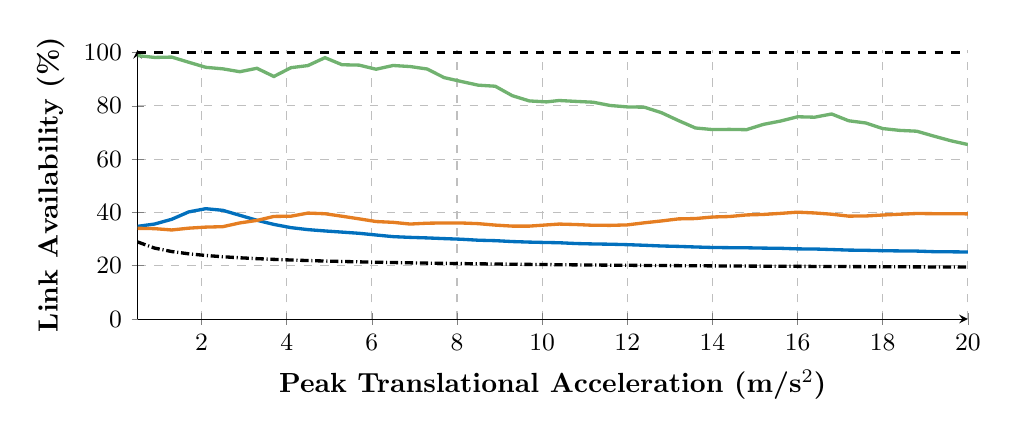
\begin{tikzpicture}
    \begin{axis}[
        width=\linewidth, height=5cm,
        xlabel={Peak Translational Acceleration (m/s$^2$)},
        ylabel={Link Availability (\%)},
        ylabel style={
            align=center
        },
        ymin=0,
        ymax=101,
    ]
        \addplot+[color=cb_blue, mark=none, solid, very thick]
            coordinates {
                (0.5, 34.788587207233697)
                (0.9, 35.660441108916025)
                (1.3, 37.43540003473295)
                (1.7, 40.208439272915996)
                (2.1, 41.412192742581695)
                (2.5, 40.79627115464352)
                (2.9, 38.931740832048078)
                (3.3, 37.069553592264327)
                (3.7, 35.51140672847211)
                (4.1, 34.302005907952299)
                (4.5, 33.559604097320445)
                (4.9, 33.058647440887846)
                (5.3, 32.625548451248946)
                (5.7, 32.180325615404385)
                (6.1, 31.540004003853813)
                (6.5, 30.925025021278771)
                (6.9, 30.648899307915183)
                (7.3, 30.448004867613228)
                (7.7, 30.183736682559729)
                (8.1, 29.953731240922004)
                (8.5, 29.583149682962841)
                (8.9, 29.414101043249094)
                (9.3, 29.080877953980892)
                (9.7, 28.872180567708892)
                (10.1, 28.727602366272002)
                (10.4, 28.634278108626706)
                (10.8, 28.338059151981945)
                (11.2, 28.181916703085925)
                (11.6, 28.082055627634841)
                (12.0, 27.914815093723668)
                (12.4, 27.688056977989646)
                (12.8, 27.418979932819809)
                (13.2, 27.263377463953915)
                (13.6, 27.043365116382208)
                (14.0, 26.857148526411766)
                (14.4, 26.784873353182785)
                (14.8, 26.738073030630499)
                (15.2, 26.616210768276719)
                (15.6, 26.550730243047148)
                (16.0, 26.330737359396498)
                (16.4, 26.286870302194476)
                (16.8, 26.085812976559318)
                (17.2, 25.874229280489722)
                (17.6, 25.798575133908198)
                (18.0, 25.650336284651704)
                (18.4, 25.563445602001284)
                (18.8, 25.50351337781964)
                (19.2, 25.283855101527315)
                (19.6, 25.229905710298613)
                (20.0, 25.158140496485441)
            };
        \addlegendentry{Baseline}
        \addplot+[color=cb_orange, mark=none, solid, very thick]
            coordinates {
                (0.5, 34.044439831638712)
                (0.9, 33.927342333126937)
                (1.3, 33.427193795757553)
                (1.7, 34.1003182622092)
                (2.1, 34.499737100101257)
                (2.5, 34.662126341051234)
                (2.9, 36.072265694634432)
                (3.3, 37.012053255407828)
                (3.7, 38.505572061305443)
                (4.1, 38.589692368046244)
                (4.5, 39.761589783583709)
                (4.9, 39.517130307154275)
                (5.3, 38.582578322786858)
                (5.7, 37.603776788502202)
                (6.1, 36.592490424863797)
                (6.5, 36.289772536183314)
                (6.9, 35.647778004220335)
                (7.3, 35.9647066368873)
                (7.7, 36.066746428970511)
                (8.1, 36.049752465340077)
                (8.5, 35.79958504300253)
                (8.9, 35.253625384464513)
                (9.3, 34.873598964987991)
                (9.7, 34.873979059698712)
                (10.1, 35.318204726847476)
                (10.4, 35.641100713380588)
                (10.8, 35.464378246163591)
                (11.2, 35.185856426442847)
                (11.6, 35.15960349848681)
                (12.0, 35.32768352719274)
                (12.4, 36.116491596669441)
                (12.8, 36.804164312660689)
                (13.2, 37.582326961145327)
                (13.6, 37.708745942233826)
                (14.0, 38.294018553489082)
                (14.4, 38.470558651785723)
                (14.8, 39.066658792802684)
                (15.2, 39.25701871377246)
                (15.6, 39.650906560322454)
                (16.0, 40.106706488624447)
                (16.4, 39.809034089292474)
                (16.8, 39.341905318913511)
                (17.2, 38.620311262927991)
                (17.6, 38.67486674659326)
                (18.0, 39.038133087598723)
                (18.4, 39.332228988065147)
                (18.8, 39.604066458032108)
                (19.2, 39.540133176522751)
                (19.6, 39.503119500823914)
                (20.0, 39.474389351077086)
            };
        \addlegendentry{IMU-Assist}
        \addplot+[color=cb_green, mark=none, solid, very thick]
            coordinates {
                (0.5, 98.864693392198305)
                (0.9, 98.159317786083548)
                (1.3, 98.296995236348593)
                (1.7, 96.359886596390538)
                (2.1, 94.461201980966834)
                (2.5, 93.883088321683672)
                (2.9, 92.809221693660646)
                (3.3, 94.096955240129958)
                (3.7, 91.026114551786662)
                (4.1, 94.316084461569631)
                (4.5, 95.115878807763224)
                (4.9, 98.082923604882311)
                (5.3, 95.425103419738832)
                (5.7, 95.281929030926932)
                (6.1, 93.741947164267486)
                (6.5, 95.143607449862287)
                (6.9, 94.747242502489797)
                (7.3, 93.82485149942498)
                (7.7, 90.588415795697287)
                (8.1, 89.144249562042077)
                (8.5, 87.758696467962679)
                (8.9, 87.358891073743195)
                (9.3, 83.811770085775038)
                (9.7, 81.844897124698306)
                (10.1, 81.481922046560527)
                (10.4, 82.004011628791048)
                (10.8, 81.666727768896081)
                (11.2, 81.359815238198479)
                (11.6, 80.133924921604645)
                (12.0, 79.603219652744556)
                (12.4, 79.494023066487983)
                (12.8, 77.456957570839975)
                (13.2, 74.487330153870019)
                (13.6, 71.698972100740605)
                (14.0, 71.103832915454277)
                (14.4, 71.167006377757971)
                (14.8, 71.058713057520137)
                (15.2, 73.056882172174767)
                (15.6, 74.290278670259042)
                (16.0, 75.90538248514828)
                (16.4, 75.739879204764406)
                (16.8, 76.946185961867627)
                (17.2, 74.403384475879037)
                (17.6, 73.573744424239834)
                (18.0, 71.475537358069033)
                (18.4, 70.792769969104015)
                (18.8, 70.481617811349778)
                (19.2, 68.645378971560518)
                (19.6, 66.902094686890607)
                (20.0, 65.486637360200575)
            };
        \addlegendentry{JIT}
        \addplot+[color=black, mark=none, densely dashdotted, very thick]
            coordinates {
                (0.5, 28.922723100170884)
                (0.9, 26.613855198751676)
                (1.3, 25.333733542045753)
                (1.7, 24.481862601570985)
                (2.1, 23.85911750262366)
                (2.5, 23.377209328589984)
                (2.9, 22.988734853082573)
                (3.3, 22.666581494386374)
                (3.7, 22.393675704265043)
                (4.1, 22.158288119378803)
                (4.5, 21.952433753598417)
                (4.9, 21.770266931392015)
                (5.3, 21.60766350567224)
                (5.7, 21.461220239419696)
                (6.1, 21.328488618791834)
                (6.5, 21.207259830366738)
                (6.9, 21.09601824689225)
                (7.3, 20.993366270578267)
                (7.7, 20.898455853574095)
                (8.1, 20.810197073347528)
                (8.5, 20.727825191476068)
                (8.9, 20.650728057491104)
                (9.3, 20.578452022094694)
                (9.7, 20.510313605591936)
                (10.1, 20.446001875872167)
                (10.4, 20.385280099721367)
                (10.8, 20.32788852118914)
                (11.2, 20.273132191965313)
                (11.6, 20.22119667184045)
                (12.0, 20.17168275705677)
                (12.4, 20.12455408277885)
                (12.8, 20.079392831598188)
                (13.2, 20.036259799758348)
                (13.6, 19.994946763186945)
                (14.0, 19.955235006480827)
                (14.4, 19.917220353140443)
                (14.8, 19.880498277636775)
                (15.2, 19.845264463624513)
                (15.6, 19.811366692881506)
                (16.0, 19.778628350527466)
                (16.4, 19.746993365826736)
                (16.8, 19.71654207456119)
                (17.2, 19.687053950355253)
                (17.6, 19.65855452265345)
                (18.0, 19.630884326386713)
                (18.4, 19.60411888177984)
                (18.8, 19.578197911525937)
                (19.2, 19.55306450615375)
                (19.6, 19.52862014742107)
                (20.0, 19.504897237299506)
            };
        \addlegendentry{No Alignment (Static)}
        \addplot+[color=cb_black, mark=none, dashed, very thick]
            coordinates {
                (0.5, 100.0)
                (0.9, 100.0)
                (1.3, 100.0)
                (1.7, 100.0)
                (2.1, 100.0)
                (2.5, 100.0)
                (2.9, 100.0)
                (3.3, 100.0)
                (3.7, 100.0)
                (4.1, 100.0)
                (4.5, 100.0)
                (4.9, 100.0)
                (5.3, 100.0)
                (5.7, 100.0)
                (6.1, 100.0)
                (6.5, 100.0)
                (6.9, 100.0)
                (7.3, 100.0)
                (7.7, 100.0)
                (8.1, 100.0)
                (8.5, 100.0)
                (8.9, 100.0)
                (9.3, 100.0)
                (9.7, 100.0)
                (10.1, 100.0)
                (10.4, 100.0)
                (10.8, 100.0)
                (11.2, 100.0)
                (11.6, 100.0)
                (12.0, 100.0)
                (12.4, 100.0)
                (12.8, 100.0)
                (13.2, 100.0)
                (13.6, 100.0)
                (14.0, 100.0)
                (14.4, 100.0)
                (14.8, 100.0)
                (15.2, 100.0)
                (15.6, 100.0)
                (16.0, 100.0)
                (16.4, 100.0)
                (16.8, 100.0)
                (17.2, 100.0)
                (17.6, 100.0)
                (18.0, 100.0)
                (18.4, 100.0)
                (18.8, 100.0)
                (19.2, 100.0)
                (19.6, 100.0)
                (20.0, 100.0)
            };
        \addlegendentry{Theoretical Max}
        \legend{}
    \end{axis}
\end{tikzpicture}
        \vspace{-25pt}
        \caption{Link Availability vs. Peak translational acceleration}
        \label{fig:translationalLinkAvail}
    \end{subfigure}
    \caption{Link availability ($\mathrm{SNR} \geq 18.8$~dB, 64-QAM threshold) under Ideal Mechanical vs.\ peak rotational~(a) and translational~(b) acceleration. Complements Figs.~\ref{fig:trans_sim_rate} and~\ref{fig:rot_sim_rate} by showing usability rather than mean capacity.}
    \label{fig:accelLinkAvail}
    \vspace{-5pt}
\end{figure}

The link availability under the Ideal Mechanical model is quantified in Fig.~\ref{fig:accelLinkAvail}. In the rotational case (Fig.~\ref{fig:rotionalLinkAvail}), Hierarchical Search falls below 5\% above \SI{15}{deg/s^2}, offering no improvement over the static reference. IMU-Assist begins at 100\% but drops below 50\% by \SI{43}{deg/s^2} and converges to the Hierarchical Search floor above \SI{170}{deg/s^2}, as the AP's uncoordinated scanning negates the UE's local correction. JIT holds 100\% up to \SI{29}{deg/s^2}, remains above 80\% at \SI{72}{deg/s^2}, and maintains a usable link ($>$40\%) up to \SI{200}{deg/s^2}. These results demonstrate that compared to single-node correction, end-to-end node synchronization sustains usable link availability across an approximately \rev{$5\times$} wider range of rotational accelerations under human-scale conditions.

In the translational case (Fig.~\ref{fig:translationalLinkAvail}), Hierarchical Search and IMU-Assist plateau between 25--40\% across the full acceleration range, neither reliably supporting 64-QAM. JIT's availability declines gradually at higher accelerations as the beam residence time shrinks, but remains above 65\% at \SI{20}{m/s^2}. The reactive methods, by contrast, stay flat at 25--40\% regardless of acceleration, as their search cannot converge before the UE exits the beam.



%-------------------------------------------------------------------%
\subsection*{Effects of Link Geometry on Mobile Performance}

We next isolate the effect of link geometry by fixing the motion profile and varying two parameters: initial separation distance (\SIrange{1}{20}{m}) during a translational pass-by (\SI{1.5}{m} displacement, \SI{3.0}{m/s^2} peak acceleration) and total angular displacement (\SIrange{1}{120}{\degree}) during a rotational turn.

\begin{figure}[h!]
    \centering
    \begin{subfigure}{0.495\linewidth}
        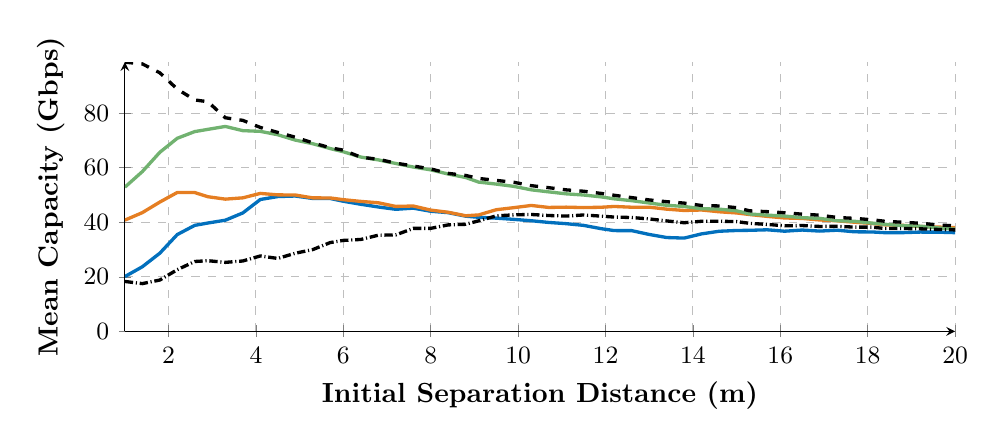
\begin{tikzpicture}
    \begin{axis}[
        width=\linewidth, height=5cm,
        xlabel={Initial Separation Distance (m)},
        ylabel={Mean Capacity (Gbps)},
        legend style={font=\small},
        ymin=0,
    ]
        \addplot+[color=cb_blue, mark=none, solid, very thick]
            coordinates {
                (1.0, 20.073056218598495) (1.4, 23.675006960359873) (1.8, 28.648010423396883) (2.2, 35.490574098514287) (2.6, 38.856536787612072) (2.9, 39.713510526149783) (3.3, 40.748004934610556) (3.7, 43.415820376988854) (4.1, 48.337418096558217) (4.5, 49.409475133891441) (4.9, 49.613318982893574) (5.3, 48.714228364377938) (5.7, 48.709504954552635) (6.0, 47.689484351174208) (6.4, 46.590071431630115) (6.8, 45.594405258207026) (7.2, 44.74041649277099) (7.6, 45.164062631135891) (8.0, 44.02489451151731) (8.4, 43.513332037132173) (8.8, 42.22014933748531) (9.1, 41.801432817714819) (9.5, 41.501215071368669) (9.9, 41.056205328707748) (10.3, 40.550482941295883) (10.7, 39.925952571941771) (11.1, 39.478213424384286) (11.5, 38.844451825313982) (11.9, 37.640746786090432) (12.2, 36.941627352151116) (12.6, 36.915668921438915) (13.0, 35.522264240010628) (13.4, 34.392095607751962) (13.8, 34.191312084099785) (14.2, 35.73481942209694) (14.6, 36.69130837029455) (15.0, 36.975241217937196) (15.3, 37.039376657872467) (15.7, 37.231671149818908) (16.1, 36.714137481967775) (16.5, 37.137409221878428) (16.9, 36.755562072802483) (17.3, 37.074173431491459) (17.7, 36.491083907151172) (18.1, 36.434935455327633) (18.4, 36.169177945629478) (18.8, 36.184507438664014) (19.2, 36.391001996796241) (19.6, 36.36225998972953) (20.0, 36.179556077601049)
            };
        \addlegendentry{Baseline}
        \addplot+[color=cb_orange, mark=none, solid, very thick]
            coordinates {
                (1.0, 40.76652478281693) (1.4, 43.524462475954024) (1.8, 47.394295836297474) (2.2, 50.916290343234323) (2.6, 50.872237146604235) (2.9, 49.354528756082935) (3.3, 48.469180177502174) (3.7, 48.946435486826765) (4.1, 50.570504587094433) (4.5, 50.03656780998854) (4.9, 49.981117184568625) (5.3, 48.930766039958939) (5.7, 48.908016633298068) (6.0, 48.271690474517577) (6.4, 47.642148148852854) (6.8, 47.133535124571566) (7.2, 45.798762351546692) (7.6, 45.949963537071042) (8.0, 44.457785839865394) (8.4, 43.650448685743008) (8.8, 42.368455671811226) (9.1, 42.691989756530823) (9.5, 44.593959016078976) (9.9, 45.341749678047357) (10.3, 46.155029208558837) (10.7, 45.423655008018777) (11.1, 45.532057732671475) (11.5, 45.370733156986319) (11.9, 45.496172558773729) (12.2, 45.782572174831778) (12.6, 45.507370076979555) (13.0, 45.521359505764266) (13.4, 44.795495351902218) (13.8, 44.312817545775097) (14.2, 44.487609114175264) (14.6, 43.837755725165223) (15.0, 43.401925769669504) (15.3, 42.822048047341966) (15.7, 42.144759693112306) (16.1, 41.562457873599904) (16.5, 41.393020011683554) (16.9, 40.832461770239021) (17.3, 40.523488459728988) (17.7, 39.995532145987013) (18.1, 39.539946576511781) (18.4, 39.032254032324097) (18.8, 38.868309749480666) (19.2, 38.436811731999903) (19.6, 38.230064594431909) (20.0, 38.043454240546282)
            };
        \addlegendentry{IMU-Assist}
        \addplot+[color=cb_green, mark=none, solid, very thick]
            coordinates {
                (1.0, 52.846642781282725) (1.4, 58.565608996273049) (1.8, 65.634657482635944) (2.2, 70.78488617376432) (2.6, 73.239037314150238) (2.9, 74.051309446843746) (3.3, 75.120981649552107) (3.7, 73.578840282127615) (4.1, 73.326016648590922) (4.5, 72.075932366227619) (4.9, 70.11934313209683) (5.3, 68.78575449786547) (5.7, 67.01799430299506) (6.0, 65.83012326286021) (6.4, 63.898388047320395) (6.8, 62.857828917924444) (7.2, 61.54927359404272) (7.6, 60.244559177262126) (8.0, 59.199439716959766) (8.4, 57.671799194657616) (8.8, 56.3964394814954) (9.1, 54.709186964700706) (9.5, 53.984537459253204) (9.9, 53.15493283020499) (10.3, 51.88790125897015) (10.7, 51.13453255453932) (11.1, 50.41328737327734) (11.5, 49.97511953107009) (11.9, 49.298350221640106) (12.2, 48.57978389762144) (12.6, 47.90148465244279) (13.0, 47.04931296117521) (13.4, 46.20900805672075) (13.8, 45.77994405750061) (14.2, 44.95601545554274) (14.6, 44.81013647262587) (15.0, 44.18079218376198) (15.3, 43.02245188853366) (15.7, 42.604249566809) (16.1, 42.25635953571973) (16.5, 41.676045448258556) (16.9, 41.4260474595213) (17.3, 40.55563894995898) (17.7, 40.35160734808875) (18.1, 39.67954202625424) (18.4, 39.23960296935367) (18.8, 38.762600882653686) (19.2, 38.55964532479593) (19.6, 37.950317740844795) (20.0, 37.4635891765508)
            };
        \addlegendentry{JIT}
        \addplot+[color=black, mark=none, densely dashdotted, very thick]
            coordinates {
                (1.0, 18.288748447986936) (1.4, 17.498038326935401) (1.8, 18.810054021611485) (2.2, 22.601805749196121) (2.6, 25.604282674193133) (2.9, 25.898507266994965) (3.3, 25.287214046457688) (3.7, 25.793822165618142) (4.1, 27.637175738152557) (4.5, 26.726974990276592) (4.9, 28.636698587445672) (5.3, 29.968781817456534) (5.7, 32.547200140486758) (6.0, 33.334001284630737) (6.4, 33.686905625347556) (6.8, 35.242367767202147) (7.2, 35.358920570410355) (7.6, 37.742053197876267) (8.0, 37.758870568815773) (8.4, 39.02677536461097) (8.8, 39.239815547249364) (9.1, 40.542018458422191) (9.5, 42.334784935573879) (9.9, 42.716964122292943) (10.3, 42.843816884393789) (10.7, 42.46470487176618) (11.1, 42.26028932171522) (11.5, 42.669063750767691) (11.9, 42.233962729811388) (12.2, 41.895878222278263) (12.6, 41.730214743433947) (13.0, 41.211076758034586) (13.4, 40.479594374674804) (13.8, 39.818495316444597) (14.2, 40.357695654245987) (14.6, 40.366942252830505) (15.0, 40.237848441692492) (15.3, 39.595122420028765) (15.7, 39.204851129914012) (16.1, 38.696438402207178) (16.5, 38.792046101856592) (16.9, 38.459874473032912) (17.3, 38.502491704609142) (17.7, 38.214771080370902) (18.1, 38.205306586608458) (18.4, 37.691230319074684) (18.8, 37.711995299126677) (19.2, 37.586693841310606) (19.6, 37.368875288032832) (20.0, 37.193775393125804)
            };
        \addlegendentry{No Alignment (Static)}
        \addplot+[color=cb_black, mark=none, dashed, very thick]
            coordinates {
                (1.0, 98.68097422801216) (1.4, 98.05509255866103) (1.8, 94.79263483783078) (2.2, 88.80442006043201) (2.6, 84.8355776245838) (2.9, 84.18486451881974) (3.3, 78.2974111474879) (3.7, 77.34765706015818) (4.1, 74.75923961650574) (4.5, 72.9199069828905) (4.9, 71.18649978844023) (5.3, 69.09925321366272) (5.7, 67.3008427291246) (6.0, 66.43374095902605) (6.4, 63.84451925812291) (6.8, 63.09061997135741) (7.2, 61.67166617463301) (7.6, 60.630632558507024) (8.0, 59.54346303716397) (8.4, 57.9176383449691) (8.8, 57.154963710650094) (9.1, 56.058156985141004) (9.5, 55.33719168849453) (9.9, 54.655785930851195) (10.3, 53.415630727440885) (10.7, 52.67332376191872) (11.1, 51.87369497895388) (11.5, 51.35988540359794) (11.9, 50.57102043964827) (12.2, 49.88893388819058) (12.6, 49.03487215449932) (13.0, 48.177452637347734) (13.4, 47.528426750628675) (13.8, 47.013784820942966) (14.2, 46.13638036156136) (14.6, 45.96779729885152) (15.0, 45.3495924209777) (15.3, 44.186212153912194) (15.7, 43.87917841782792) (16.1, 43.47569101129677) (16.5, 42.96708513272225) (16.9, 42.595122248191934) (17.3, 41.752090169536395) (17.7, 41.42431379252635) (18.1, 40.907653535870836) (18.4, 40.33949302896137) (18.8, 40.00260745626302) (19.2, 39.632326763336344) (19.6, 39.0497033367617) (20.0, 38.64496975281596)
            };
        \addlegendentry{Theoretical Max}
        \legend{}
    \end{axis}
\end{tikzpicture}
        \vspace{-25pt}
        \caption{Mean Capacity vs. Separation Distance}
        \label{fig:dist_rate}
    \end{subfigure}
    \hfill
    \begin{subfigure}{0.495\linewidth}
        \include{Figures/Fig6b}
        \vspace{-25pt}
        \caption{Capacity CoV vs. Separation Distance}
        \label{fig:dist_cov}
    \end{subfigure}
    \caption{Effect of initial AP--UE separation (1--20~m) on a fixed translational pass-by ($D_{traversed} = 1.5$~m, $3.0$~m/s$^2$ peak), Ideal Mechanical. Performance converges beyond ${\sim}10$~m as path loss, not alignment, becomes the limiting factor.}
    \vspace{-5pt}
\end{figure}

Mean capacity as a function of initial separation distance (\SIrange{1}{20}{m}) is shown in Fig.~\ref{fig:dist_rate}. At close range, the fixed \SI{1.5}{m} displacement corresponds to a large angular change relative to the AP, generating angular velocities that overwhelm reactive tracking. This is evident at \SI{1}{m}, where Hierarchical Search achieves only \SI{20}{Gbps}, slightly above the static reference of \SI{18}{Gbps}, while IMU-Assist and JIT reach \SI{41}{Gbps} and \SI{53}{Gbps}, respectively. A crossover occurs at $\approx$\SI{4.5}{m}: beyond this distance, angular rates decrease enough for Hierarchical Search to recover the link, reaching \SI{49}{Gbps}. The performance gap narrows further beyond \SI{10}{m} as path loss reduces the link budget, and all algorithms converge to \SIrange{37}{39}{Gbps} by \SI{20}{m}, where alignment accuracy is no longer the limiting factor.

The capacity CoV (Fig.~\ref{fig:dist_cov}) complements this view. At \SI{1}{m}, Hierarchical Search exhibits a CoV of 2.0, indicating highly erratic capacity, while IMU-Assist and JIT reduce this to 0.57 and 0.48. As separation increases to \SI{4.5}{m}, JIT achieves near-zero CoV (0.047) while Hierarchical Search and IMU-Assist settle at 0.25 and 0.20, respectively. JIT maintains CoV below 0.02 across all distances beyond \SI{5}{m}, confirming stable link behavior regardless of link geometry.

\begin{figure*}[ht!]
    \centering
    \begin{subfigure}[t]{0.49\textwidth}
        \vspace{0pt}
        \centering
        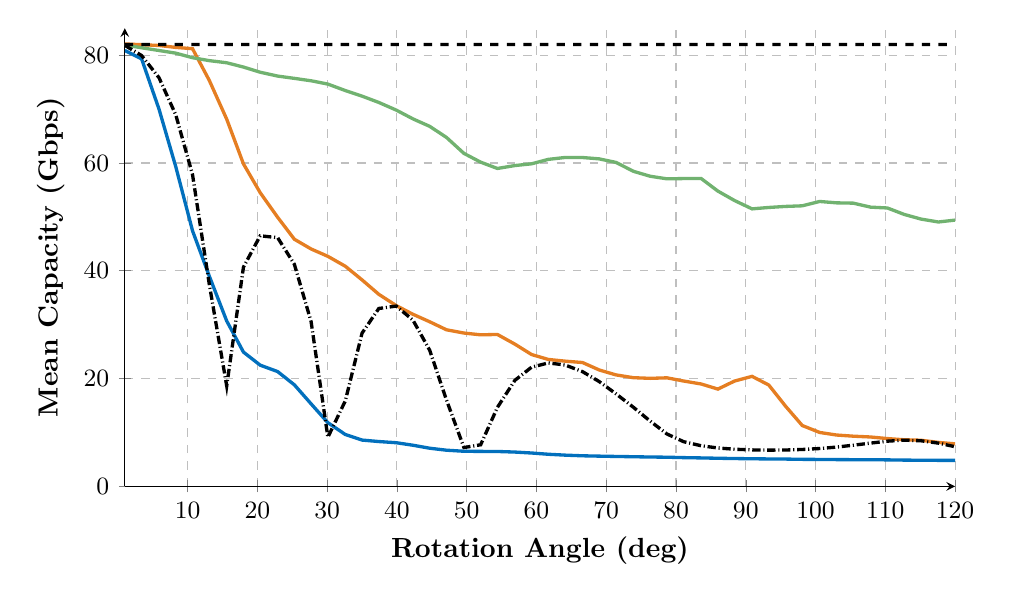
\begin{tikzpicture}
    \begin{axis}[
        width=\linewidth, height=7.4cm,
        xlabel={Rotation Angle (deg)},
        ylabel={Mean Capacity (Gbps)},
        legend style={font=\small},
        legend columns=2,
        ymin=0,
        ymax=85
    ]
        \addplot+[color=cb_blue, mark=none, solid, very thick]
            coordinates {
                (1.0, 80.875350599427989)
                (3.4, 79.31594089943178)
                (5.9, 69.971046290208193)
                (8.3, 59.300872319542421)
                (10.7, 47.419150399983003)
                (13.1, 39.021437126801594)
                (15.6, 30.682979490746696)
                (18.0, 24.910713175457492)
                (20.4, 22.486931110064514)
                (22.9, 21.296496524905614)
                (25.3, 18.832302723509432)
                (27.7, 15.303597949307994)
                (30.1, 11.815637790480327)
                (32.6, 9.624689986161366)
                (35.0, 8.5893432901649547)
                (37.4, 8.316401499412823)
                (39.9, 8.0969176382221644)
                (42.3, 7.6313154696982775)
                (44.7, 7.0748896944527946)
                (47.1, 6.7093536439993962)
                (49.6, 6.5128024297205629)
                (52.0, 6.4877006787111773)
                (54.4, 6.4721171468486256)
                (56.9, 6.3643735179337373)
                (59.3, 6.187846183050139)
                (61.7, 5.9560031295594502)
                (64.1, 5.7939769181796912)
                (66.6, 5.6717983438058592)
                (69.0, 5.6076073768508401)
                (71.4, 5.5507020156522469)
                (73.9, 5.497011718905024)
                (76.3, 5.4459541872031609)
                (78.7, 5.4090411092465827)
                (81.1, 5.3318194333386533)
                (83.6, 5.2775418392141757)
                (86.0, 5.2149909781364521)
                (88.4, 5.1630328020243965)
                (90.9, 5.1201232741493188)
                (93.3, 5.0880736858996451)
                (95.7, 5.0636701344437682)
                (98.1, 5.0147578373529829)
                (100.6, 4.9963751299479338)
                (103.0, 4.9670628867637863)
                (105.4, 4.9507418475627905)
                (107.9, 4.9414474273467919)
                (110.3, 4.9168329042367738)
                (112.7, 4.8712292993673154)
                (115.1, 4.8488400981739126)
                (117.6, 4.8269343309050532)
                (120.0, 4.819651635196827)
            };
        \addlegendentry{Baseline}
        \addplot+[color=cb_orange, mark=none, solid, very thick]
            coordinates {
                (1.0, 82.080349941563568)
                (3.4, 81.944577964361585)
                (5.9, 81.796534493342932)
                (8.3, 81.441340276280499)
                (10.7, 81.199037427702692)
                (13.1, 75.326098516257616)
                (15.6, 68.123844402979827)
                (18.0, 59.832359435851131)
                (20.4, 54.484866430403464)
                (22.9, 49.9267268298292)
                (25.3, 45.846787573029694)
                (27.7, 44.041366724697639)
                (30.1, 42.67582865747692)
                (32.6, 40.839621070207713)
                (35.0, 38.305655990400439)
                (37.4, 35.632485624372848)
                (39.9, 33.538828874570257)
                (42.3, 31.924246948286406)
                (44.7, 30.534307757167849)
                (47.1, 29.051312590704754)
                (49.6, 28.446085222357873)
                (52.0, 28.1176754875382)
                (54.4, 28.181327570886005)
                (56.9, 26.393023475158699)
                (59.3, 24.458933545013739)
                (61.7, 23.547421172385672)
                (64.1, 23.232529480895803)
                (66.6, 22.97486971063471)
                (69.0, 21.59176475542402)
                (71.4, 20.678716502895004)
                (73.9, 20.162018131099771)
                (76.3, 20.04186102011786)
                (78.7, 20.13848285058441)
                (81.1, 19.541487973612078)
                (83.6, 18.99719636257495)
                (86.0, 18.047154077849303)
                (88.4, 19.544589146340645)
                (90.9, 20.408672599733407)
                (93.3, 18.800547160102557)
                (95.7, 14.878705930434391)
                (98.1, 11.286415210020754)
                (100.6, 10.001337757036293)
                (103.0, 9.5271149864647171)
                (105.4, 9.31092944458217)
                (107.9, 9.1599537400659692)
                (110.3, 8.8658693203021883)
                (112.7, 8.646232230887934)
                (115.1, 8.5586023205662229)
                (117.6, 8.1588060306845112)
                (120.0, 7.8872232654343941)
            };
        \addlegendentry{IMU-Assist}
        \addplot+[color=cb_green, mark=none, solid, very thick]
            coordinates {
                (1.0, 81.89540782622116)
                (3.4, 81.371785025549883)
                (5.9, 80.865073149365628)
                (8.3, 80.372680126456487)
                (10.7, 79.528269771537467)
                (13.1, 78.988191483468995)
                (15.6, 78.591371817538302)
                (18.0, 77.79406433295317)
                (20.4, 76.836241430823364)
                (22.9, 76.122558950967658)
                (25.3, 75.695401464574317)
                (27.7, 75.249662132313247)
                (30.1, 74.634316588945367)
                (32.6, 73.435522680157561)
                (35.0, 72.398110290388999)
                (37.4, 71.229181240152187)
                (39.9, 69.810453909512887)
                (42.3, 68.177959540801893)
                (44.7, 66.790813802589128)
                (47.1, 64.739715797721445)
                (49.6, 61.778905963801741)
                (52.0, 60.150420843921701)
                (54.4, 58.980582485033175)
                (56.9, 59.520299709243389)
                (59.3, 59.844100971306098)
                (61.7, 60.669160291829947)
                (64.1, 61.018071368352125)
                (66.6, 61.014023923833037)
                (69.0, 60.756415883359558)
                (71.4, 60.103360483948691)
                (73.9, 58.449831743453494)
                (76.3, 57.535411915450652)
                (78.7, 57.057635138831479)
                (81.1, 57.106554138963929)
                (83.6, 57.118972753976429)
                (86.0, 54.782045443266739)
                (88.4, 53.024902061226875)
                (90.9, 51.483241374559782)
                (93.3, 51.74614554895345)
                (95.7, 51.936997712594362)
                (98.1, 52.052161875457465)
                (100.6, 52.85798218203945)
                (103.0, 52.602048965447537)
                (105.4, 52.54532990097146)
                (107.9, 51.802038637730618)
                (110.3, 51.649978877187884)
                (112.7, 50.457442682640469)
                (115.1, 49.59529054431372)
                (117.6, 49.048860307034744)
                (120.0, 49.398569688940505)
            };
        \addlegendentry{JIT}
        \addplot+[color=black, mark=none, densely dashdotted, very thick]
            coordinates {
                (1.0, 81.81407730233013)
                (3.4, 79.93455246394336)
                (5.9, 75.81170885125118)
                (8.3, 68.92368374783945)
                (10.7, 57.84253340983341)
                (13.1, 37.5190630402623)
                (15.6, 18.632437765215688)
                (18.0, 40.68580053927078)
                (20.4, 46.48593195987912)
                (22.9, 46.147492371852884)
                (25.3, 41.19298468645134)
                (27.7, 30.543909951780616)
                (30.1, 9.11091823017484)
                (32.6, 15.860232595368236)
                (35.0, 28.432392799922912)
                (37.4, 33.00228075971154)
                (39.9, 33.44857855974167)
                (42.3, 30.83551992713738)
                (44.7, 25.243538140830548)
                (47.1, 16.02455423248359)
                (49.6, 7.2038982700002)
                (52.0, 7.719164088952767)
                (54.4, 14.65077701445825)
                (56.9, 19.666629286956955)
                (59.3, 22.11593004099943)
                (61.7, 22.899220172092114)
                (64.1, 22.516075202740964)
                (66.6, 21.284958054216613)
                (69.0, 19.43570230278142)
                (71.4, 17.166388244219405)
                (73.9, 14.664527865411737)
                (76.3, 12.106214859335058)
                (78.7, 9.717564889607944)
                (81.1, 8.28356425125056)
                (83.6, 7.534996028299513)
                (86.0, 7.122343492947932)
                (88.4, 6.889668019356687)
                (90.9, 6.7665452531226515)
                (93.3, 6.722369358392766)
                (95.7, 6.747412395466279)
                (98.1, 6.844173861600484)
                (100.6, 7.0214979983650485)
                (103.0, 7.287328732332879)
                (105.4, 7.635316497417764)
                (107.9, 8.02829666034476)
                (110.3, 8.383783920314944)
                (112.7, 8.570944306793603)
                (115.1, 8.462497861787059)
                (117.6, 8.022240339765782)
                (120.0, 7.356281716521055)
            };
        \addlegendentry{Static}
        \addplot+[color=cb_black, mark=none, dashed, very thick]
            coordinates {
                (1.0, 81.98194012674426)
                (3.4, 81.98194076566816)
                (5.9, 81.98194033013311)
                (8.3, 81.98194129638972)
                (10.7, 81.98194201787368)
                (13.1, 81.9819414128587)
                (15.6, 81.98194089143364)
                (18.0, 81.98194108958693)
                (20.4, 81.98194064937952)
                (22.9, 81.98193967701685)
                (25.3, 81.9819390427902)
                (27.7, 81.98193908784225)
                (30.1, 81.98193994928012)
                (32.6, 81.98194016979966)
                (35.0, 81.98194074368875)
                (37.4, 81.98194125194688)
                (39.9, 81.98194191429961)
                (42.3, 81.98194122948925)
                (44.7, 81.9819412195923)
                (47.1, 81.98194160507181)
                (49.6, 81.98194167000185)
                (52.0, 81.98194265546617)
                (54.4, 81.98194275209777)
                (56.9, 81.98194231647683)
                (59.3, 81.98194316247262)
                (61.7, 81.98194290370176)
                (64.1, 81.98194299466645)
                (66.6, 81.98194297606358)
                (69.0, 81.9819431259863)
                (71.4, 81.98194264642916)
                (73.9, 81.98194314257654)
                (76.3, 81.9819442722217)
                (78.7, 81.98194335348157)
                (81.1, 81.9819431237318)
                (83.6, 81.98194244807242)
                (86.0, 81.98194298181593)
                (88.4, 81.98194338764694)
                (90.9, 81.98194393004016)
                (93.3, 81.98194481674278)
                (95.7, 81.9819455287004)
                (98.1, 81.98194538690197)
                (100.6, 81.98194497371087)
                (103.0, 81.98194494689407)
                (105.4, 81.9819458348762)
                (107.9, 81.98194606136559)
                (110.3, 81.98194641196822)
                (112.7, 81.98194679467736)
                (115.1, 81.98194608008282)
                (117.6, 81.98194600570741)
                (120.0, 81.98194592545394)
            };
        \addlegendentry{Theo. Max.}
        \legend{}
     \end{axis}
\end{tikzpicture}
        \vspace{-25pt}
        \caption{Mean Capacity}
        \label{fig:angle_rate}
    \end{subfigure}%
    \hfill
    \begin{minipage}[t]{0.49\textwidth}
        \vspace{0pt}
        \centering
        \begin{subfigure}{\linewidth}
            \include{Figures/Fig7b}
            \vspace{-25pt}
            \caption{Link Availability}
        \label{fig:angle_avail}
        \end{subfigure}
        \vfill
        \begin{subfigure}{\linewidth}
            \include{Figures/Fig7c}
            \vspace{-25pt}
            \caption{Signaling Overhead}
        \label{fig:angle_overhead}
        \end{subfigure}
    \end{minipage}

    \vspace{5 pt}

    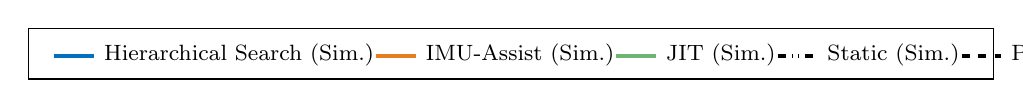
\begin{tikzpicture}
        \node [
            draw=black,
            line width=0.5pt,
            inner sep=3pt,
            rounded corners=0pt,
            align=center
        ] {
            \footnotesize
            \setlength{\tabcolsep}{0pt}
            \renewcommand{\arraystretch}{1.3}
            \begin{tabular*}{\dimexpr0.969\linewidth}{
                c @{\extracolsep{0pt}\hspace{3pt}} l
                @{\extracolsep{\fill}}
                c @{\extracolsep{0pt}\hspace{3pt}} l
                @{\extracolsep{\fill}}
                c @{\extracolsep{0pt}\hspace{3pt}} l
                @{\extracolsep{\fill}}
                c @{\extracolsep{0pt}\hspace{3pt}} l
                @{\extracolsep{\fill}}
                c @{\extracolsep{0pt}\hspace{3pt}} l
            }

                % --- ROW 1: SIMULATIONS ---
                \legline{cb_blue}{solid} & Hierarchical Search (Sim.) &
                \legline{cb_orange}{solid} & IMU-Assist (Sim.) &
                \legline{cb_green}{solid} & JIT (Sim.) &
                \legline{black}{dashdotdotted} & Static (Sim.) &
                \legline{black}{dashed} & Perfect Alignment (Sim.) \\

            \end{tabular*}
        };
    \end{tikzpicture}
    \caption{Effect of total angular displacement ($1^\circ$--$120^\circ$) at fixed rotational acceleration ($120$~deg/s$^2$), Ideal Mechanical. (c)~Overhead plateaus at ${\sim}0.39\%$ above $90^\circ$ as realignment frequency saturates.}
    \label{fig:angle_effects}
    \vspace{-5pt}
\end{figure*}

For the rotational sweep (Fig.~\ref{fig:angle_rate}), Hierarchical Search drops from \SI{81}{Gbps} to under \SI{9}{Gbps} by \SI{35}{\degree} and settles at $\approx$\SI{5}{Gbps}, again falling below the static reference due to misdirected AP scanning. IMU-Assist maintains \SI{81}{Gbps} through \SI{10}{\degree} but degrades to \SI{34}{Gbps} by \SI{40}{\degree} as the AP's uncoordinated scanning erodes the UE's correction. JIT sustains above \SI{55}{Gbps} through \SI{50}{\degree} and remains above \SI{40}{Gbps} at \SI{120}{\degree}, maintaining a capacity advantage of at least $2\times$ over IMU-Assist across the full angular range.

Link availability over the same sweep is quantified in Fig.~\ref{fig:angle_avail}. Hierarchical Search falls below 50\% by \SI{11}{\degree} and under 5\% by \SI{20}{\degree}. IMU-Assist holds 100\% through \SI{10}{\degree} but drops below 50\% by \SI{28}{\degree} and converges toward Hierarchical Search's floor above \SI{90}{\degree}. JIT maintains 100\% through \SI{30}{\degree} and remains above 40\% at \SI{120}{\degree}, extending the usable angular range by approximately $3\times$ compared to Hierarchical Search. This gain requires additional signaling, quantified in Fig.~\ref{fig:angle_effects}c. JIT overhead rises from 0.01\% at \SI{1}{\degree} to 0.23\% at \SI{35}{\degree} as the algorithm triggers more frequent realignment updates, then plateaus at $\approx$0.39\% for angles above \SI{90}{\degree}. Even at maximum rotation, this represents a negligible fraction of total channel capacity.



%-------------------------------------------------------------------%
\subsection*{Impact of Antenna Directivity on Combined Motion}

The preceding sections evaluated each motion type independently. We now combine translational (\SI{1.5}{m} displacement) and rotational (\SI{90}{\degree} turn) motion simultaneously, with acceleration escalating from (\SI{0.5}{m/s^2}, \SI{0.5}{deg/s^2}) to (\SI{5}{m/s^2}, \SI{200}{deg/s^2}). We evaluate four antenna configurations with HPBWs of \SI{13}{\degree} (\SI{21}{dBi}), \SI{9}{\degree} (\SI{27}{dBi}), \SI{4}{\degree} (\SI{34}{dBi}), and \SI{1.3}{\degree} (\SI{40}{dBi}), using link availability to assess the gain-beamwidth trade-off under mobility.

\begin{figure*}[ht!]
    \centering
    \begin{subfigure}{0.495\linewidth}
        \centering
        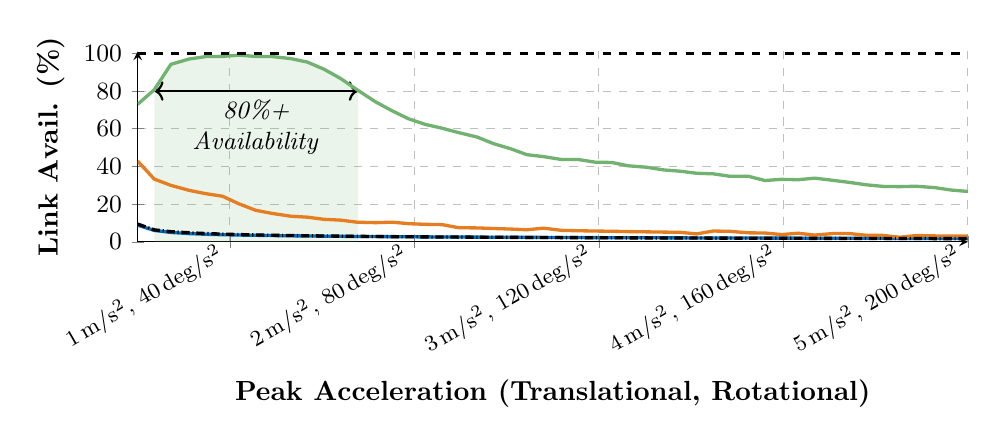
\begin{tikzpicture}
    \begin{axis}[
        width=\linewidth, height=4cm,
        xlabel={Peak Acceleration (Translational, Rotational)},
        ylabel={Link Avail. (\%)},
        legend style={font=\small},
        ymin=0,
        ymax=101,
        x tick label style={rotate=30, anchor=east, font=\footnotesize},
        xtick={0, 1, 2, 3, 4, 5},
        xticklabels={
            0,
            {1\,m/s$^2$, 40\,deg/s$^2$ },
            {2\,m/s$^2$, 80\,deg/s$^2$ },
            {3\,m/s$^2$, 120\,deg/s$^2$ },
            {4\,m/s$^2$, 160\,deg/s$^2$ },
            {5\,m/s$^2$, 200\,deg/s$^2$ }
        },
    ]
    \pgfplotsextra{
            \draw[<->, black, thick] (axis cs:0.59, 80) -- (axis cs:1.695, 80);
            
            \node[
                below,
                font=\small,
                text width=2cm,
                align=center,
                inner sep=3pt
            ] at (axis cs:1.1425, 80) {\textit{80\%+ Availability}};
        }
        \addplot+[color=cb_blue, mark=none, solid, very thick]
            coordinates {
                (0.5, 8.905539442812124)
                (0.59, 6.079862332858859)
                (0.68, 5.019555846448388)
                (0.78, 4.4083610740523165)
                (0.87, 4.032316657885606)
                (0.96, 3.8119310453856263)
                (1.05, 3.6407365324344085)
                (1.14, 3.490535693584253)
                (1.23, 3.3571956977419517)
                (1.33, 3.2308853968041404)
                (1.42, 3.1299560983061427)
                (1.51, 3.0406002378362875)
                (1.6, 2.958904130274587)
                (1.69, 2.884774026437333)
                (1.79, 2.821973946131555)
                (1.88, 2.7613405305214087)
                (1.97, 2.7073627756953402)
                (2.06, 2.6564667104473485)
                (2.15, 2.6089042519478447)
                (2.24, 2.5664664824558683)
                (2.34, 2.52639874105317)
                (2.43, 2.4882851035513527)
                (2.52, 2.448321906293164)
                (2.61, 2.408550726515382)
                (2.7, 2.3685898139453583)
                (2.8, 2.328499498118966)
                (2.89, 2.2934734004130926)
                (2.98, 2.260463086757481)
                (3.07, 2.2271238139205134)
                (3.16, 2.1982924570426845)
                (3.26, 2.1717737735479785)
                (3.35, 2.1464413364801054)
                (3.44, 2.1221386011809966)
                (3.53, 2.098663037681373)
                (3.62, 2.076102986770527)
                (3.71, 2.0542354716816322)
                (3.81, 2.0331465715348758)
                (3.9, 2.012701015760699)
                (3.99, 1.9930023525553076)
                (4.08, 1.97401608483714)
                (4.17, 1.9555828064666696)
                (4.27, 1.9376450152996723)
                (4.36, 1.920312759515018)
                (4.45, 1.9034371840431388)
                (4.54, 1.8871071402321564)
                (4.63, 1.871107938081407)
                (4.72, 1.85561317139168)
                (4.82, 1.840366967750356)
                (4.91, 1.8255334079200036)
                (5.0, 1.8110810843396323)
            };
        \addlegendentry{Baseline}
        \addplot+[color=cb_orange, mark=none, solid, very thick]
            coordinates {
                (0.5, 42.855309431755494)
                (0.59, 33.32130012298278)
                (0.68, 29.982116474416422)
                (0.78, 27.313114896179485)
                (0.87, 25.568776905383)
                (0.96, 24.215899744585364)
                (1.05, 20.14168088400369)
                (1.14, 16.75182376106148)
                (1.23, 15.085249985529163)
                (1.33, 13.614627212837002)
                (1.42, 13.11328393378069)
                (1.51, 11.968727964288703)
                (1.6, 11.540929764795418)
                (1.69, 10.428324933859944)
                (1.79, 10.209647297082222)
                (1.88, 10.452210167597034)
                (1.97, 9.655923511650753)
                (2.06, 9.305030249931749)
                (2.15, 9.16235328189037)
                (2.24, 7.51900478487151)
                (2.34, 7.407038829290076)
                (2.43, 7.0900957585648765)
                (2.52, 6.809745539576191)
                (2.61, 6.442718489055303)
                (2.7, 7.278396819684479)
                (2.8, 6.101465655832021)
                (2.89, 5.910978727865072)
                (2.98, 5.7520348486056205)
                (3.07, 5.637018045720221)
                (3.16, 5.459016488332479)
                (3.26, 5.323653465313692)
                (3.35, 5.192386374409357)
                (3.44, 5.083611128250367)
                (3.53, 4.225670278376386)
                (3.62, 5.763591494977003)
                (3.71, 5.597159638273408)
                (3.81, 4.807686593561102)
                (3.9, 4.706630729641425)
                (3.99, 3.8925074655632805)
                (4.08, 4.588705070210367)
                (4.17, 3.611792757280834)
                (4.27, 4.42952855943158)
                (4.36, 4.398336929941931)
                (4.45, 3.500593663519581)
                (4.54, 3.4417859410594707)
                (4.63, 2.455376719555776)
                (4.72, 3.37352497480405)
                (4.82, 3.1750402195943277)
                (4.91, 3.1262310911143727)
                (5.0, 3.117715451859537)
            };
        \addlegendentry{IMU-Assist}
        \addplot+[color=cb_green, mark=none, solid, very thick, name path=jit_line]
             coordinates {
                (0.5, 72.960659212997754)
                (0.59, 80.685516957776727)
                (0.68, 94.177789812786315)
                (0.78, 97.015776106268035)
                (0.87, 98.289442413447333)
                (0.96, 98.393646235243523)
                (1.05, 99.029153127659441)
                (1.14, 98.36670545641185)
                (1.23, 98.282903299608122)
                (1.33, 97.217986725135376)
                (1.42, 95.363588098613405)
                (1.51, 91.594987406765824)
                (1.6, 86.674886605302646)
                (1.69, 80.629357883125309)
                (1.79, 74.240558275005625)
                (1.88, 69.494891778499962)
                (1.97, 65.205480946144888)
                (2.06, 62.288500615061444)
                (2.15, 60.287884973079215)
                (2.24, 57.960820479702875)
                (2.34, 55.595190215799292)
                (2.43, 52.063571555645311)
                (2.52, 49.463014941147804)
                (2.61, 46.239818095229857)
                (2.7, 45.230344736225334)
                (2.8, 43.654321737178201)
                (2.89, 43.65372194064809)
                (2.98, 42.280822105938519)
                (3.07, 42.121192629002444)
                (3.16, 40.352043396687243)
                (3.26, 39.583906713352746)
                (3.35, 38.187281476524184)
                (3.44, 37.498816013301173)
                (3.53, 36.399752152468324)
                (3.62, 36.089496367405339)
                (3.71, 34.799729349899337)
                (3.81, 34.805452997223696)
                (3.9, 32.55457321606184)
                (3.99, 33.173158962381301)
                (4.08, 32.965869551838992)
                (4.17, 33.804197060622286)
                (4.27, 32.639200482965634)
                (4.36, 31.521462857891994)
                (4.45, 30.267412452830964)
                (4.54, 29.430195720188991)
                (4.63, 29.305748173824732)
                (4.72, 29.501875756008129)
                (4.82, 28.787681979475554)
                (4.91, 27.493289413770011)
                (5.0, 26.748232872834205)
            };
        \addlegendentry{JIT}
        \addplot+[color=black, mark=none, densely dashdotted, very thick]
            coordinates {
                (0.5, 9.452896624057995)
                (0.59, 6.390904695367165)
                (0.68, 5.4090855069092365)
                (0.78, 4.829955950361346)
                (0.87, 4.427464372454028)
                (0.96, 4.123593601893363)
                (1.05, 3.8821424525678743)
                (1.14, 3.683393815055909)
                (1.23, 3.51564935981031)
                (1.33, 3.3713716168811696)
                (1.42, 3.2453520954221653)
                (1.51, 3.133693274850307)
                (1.6, 3.034013759528383)
                (1.69, 2.9442195300249954)
                (1.79, 2.8625624993752945)
                (1.88, 2.7880363020959256)
                (1.97, 2.7194835763190572)
                (2.06, 2.656147781796244)
                (2.15, 2.597419891209944)
                (2.24, 2.542715368886494)
                (2.34, 2.4916818443251536)
                (2.43, 2.4437549315423657)
                (2.52, 2.3987398674554723)
                (2.61, 2.3562322257995554)
                (2.7, 2.3160977711653925)
                (2.8, 2.278100849525457)
                (2.89, 2.242028477503493)
                (2.98, 2.207753831185426)
                (3.07, 2.1751514801777367)
                (3.16, 2.1439107281657765)
                (3.26, 2.1141133620160617)
                (3.35, 2.0855981944312774)
                (3.44, 2.0583769550564233)
                (3.53, 2.0322420742727125)
                (3.62, 2.0070781199199597)
                (3.71, 1.9829047481864537)
                (3.81, 1.9596133222667986)
                (3.9, 1.9372279965615473)
                (3.99, 1.9155675254381137)
                (4.08, 1.8947006433087838)
                (4.17, 1.8745058768617133)
                (4.27, 1.855010631975507)
                (4.36, 1.8361853900763585)
                (4.45, 1.817914140789311)
                (4.54, 1.8001647759030626)
                (4.63, 1.782924534681757)
                (4.72, 1.7662614695810677)
                (4.82, 1.7501603594800144)
                (4.91, 1.7344376288318473)
                (5.0, 1.7191070164469775)
            };
        \addlegendentry{No Alignment (Static)}
        \addplot+[color=cb_black, mark=none, dashed, very thick]
            coordinates {
                (0.5, 100.0)
                (0.59, 100.0)
                (0.68, 100.0)
                (0.78, 100.0)
                (0.87, 100.0)
                (0.96, 99.99999999999999)
                (1.05, 100.0)
                (1.14, 100.0)
                (1.23, 100.0)
                (1.33, 99.99999999999999)
                (1.42, 99.99999999999999)
                (1.51, 100.0)
                (1.6, 100.0)
                (1.69, 100.0)
                (1.79, 99.99999999999999)
                (1.88, 100.0)
                (1.97, 100.0)
                (2.06, 100.0)
                (2.15, 100.0)
                (2.24, 100.0)
                (2.34, 100.0)
                (2.43, 100.0)
                (2.52, 100.0)
                (2.61, 100.0)
                (2.7, 100.0)
                (2.8, 100.0)
                (2.89, 100.0)
                (2.98, 100.0)
                (3.07, 100.0)
                (3.16, 100.0)
                (3.26, 100.0)
                (3.35, 100.0)
                (3.44, 100.0)
                (3.53, 100.0)
                (3.62, 100.0)
                (3.71, 100.0)
                (3.81, 100.0)
                (3.9, 100.0)
                (3.99, 100.0)
                (4.08, 100.0)
                (4.17, 100.0)
                (4.27, 100.0)
                (4.36, 100.0)
                (4.45, 100.0)
                (4.54, 100.0)
                (4.63, 100.0)
                (4.72, 100.0)
                (4.82, 100.0)
                (4.91, 100.0)
                (5.0, 100.0)
            };
        \addlegendentry{Theoretical Max}
        \legend{}
         \path[name path=xaxis] (axis cs:0,0) -- (axis cs:5,0);
 
         \addplot[cb_green, opacity=0.15, forget plot] 
             fill between[of=jit_line and xaxis, soft clip={domain=0.59:1.695}];
    \end{axis}
\end{tikzpicture}
        \vspace{-25pt}
        \caption{13° HPBW (21 dBi)}
        \label{fig:ant_13deg}
    \end{subfigure}%
    \hfill
    \begin{subfigure}{0.495\linewidth}
        \centering
        \include{Figures/Fig8b}
        \vspace{-25pt}
        \caption{9° HPBW (27 dBi)}
        \label{fig:ant_9deg}
    \end{subfigure}
    \vspace{1em}
    \begin{subfigure}{0.495\linewidth}
        \centering
        \include{Figures/Fig8c}
        \vspace{-25pt}
        \caption{4° HPBW (34 dBi)}
        \label{fig:ant_4deg}
    \end{subfigure}%
    \hfill
    \begin{subfigure}{0.495\linewidth}
        \centering
        \include{Figures/Fig8d}
        \vspace{-25pt}
        \caption{1.3° HPBW (40 dBi)}
        \label{fig:ant_1_3deg}
    \end{subfigure}

    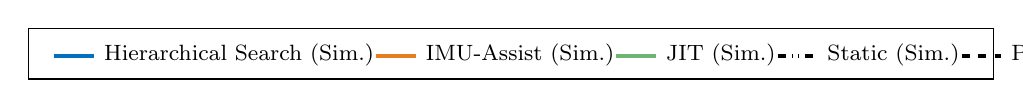
\begin{tikzpicture}
        \node [
            draw=black,
            line width=0.5pt,
            inner sep=3pt,
            rounded corners=0pt,
            align=center
        ] {
            \footnotesize
            \setlength{\tabcolsep}{0pt}
            \renewcommand{\arraystretch}{1.3} % Vertical spacing between Sim and Exp rows

            \begin{tabular*}{\dimexpr0.969\linewidth}{
                c @{\extracolsep{0pt}\hspace{3pt}} l
                @{\extracolsep{\fill}}
                c @{\extracolsep{0pt}\hspace{3pt}} l
                @{\extracolsep{\fill}}
                c @{\extracolsep{0pt}\hspace{3pt}} l
                @{\extracolsep{\fill}}
                c @{\extracolsep{0pt}\hspace{3pt}} l
                @{\extracolsep{\fill}}
                c @{\extracolsep{0pt}\hspace{3pt}} l
            }

                % --- ROW 1: SIMULATIONS ---
                \legline{cb_blue}{solid} & Hierarchical Search (Sim.) &
                \legline{cb_orange}{solid} & IMU-Assist (Sim.) &
                \legline{cb_green}{solid} & JIT (Sim.) &
                \legline{black}{dashdotdotted} & Static (Sim.) &
                \legline{black}{dashed} & Perfect Alignment (Sim.) \\

            \end{tabular*}
        };
    \end{tikzpicture}

    \caption{Combined mobility (1.5~m translation $+$ $90^\circ$ rotation, escalating acceleration) for four antenna configurations. Dashed line marks 80\% availability. The $9^\circ$ HPBW antenna yields the widest operational window, illustrating the gain--beamwidth trade-off under reaction-time constraints.}
    \label{fig:antenna_comparison}
    \vspace{-5pt}
\end{figure*}

The Hierarchical Search and IMU-Assist algorithms are ineffective across all antenna types under combined motion (Fig.~\ref{fig:antenna_comparison}). The rotational component causes Hierarchical Search to steer the AP away from the correct LoS, keeping availability below 9\% regardless of beamwidth. IMU-Assist peaks at 43\% with the \SI{13}{\degree} antenna but falls below 10\% above \SI{2}{m/s^2} and \SI{80}{deg/s^2} for all configurations.

JIT reveals a trade-off between gain and beamwidth. With the \SI{13}{\degree} antenna (Fig.~\ref{fig:ant_13deg}), the wide beam relaxes pointing requirements, but the lower gain (\SI{21}{dBi}) limits the SNR margin. JIT achieves $>$80\% availability only between \SIrange{0.6}{1.7}{m/s^2} before transient pointing errors push SNR below the \SI{18.8}{dB} threshold. The \SI{9}{\degree} antenna (Fig.~\ref{fig:ant_9deg}) provides the best balance: its higher gain (\SI{27}{dBi}) buffers against misalignment, extending the $>$80\% availability window to \SIrange{0.55}{2.85}{m/s^2} and sustaining above 63\% even at maximum acceleration.

With the \SI{4}{\degree} antenna (Fig.~\ref{fig:ant_4deg}), the $>$80\% window narrows to 0.58--1.2\,m/s$^2$ as the tighter beam demands higher pointing precision than the algorithm's reaction time can guarantee. The \SI{1.3}{\degree} antenna (Fig.~\ref{fig:ant_1_3deg}) restricts this further to 0.5--0.9\,m/s$^2$, with availability dropping below 80\% before reaching 1\,m/s$^2$. Despite their higher gain (34--40\,dBi), the angular displacement during the system's reaction latency exceeds the beamwidth, negating the link budget advantage. These results show that each mobility profile imposes a minimum usable beamwidth, and that selecting the right antenna requires jointly considering gain, control latency, and expected user motion.



%-------------------------------------------------------------------%
%-------------------------------------------------------------------%
%-------------------------------------------------------------------%
\section*{Discussion}

The above results characterize mobile sub-THz link performance as a function of link geometry, motion type and severity, and beam steering hardware, comparing four beam realignment strategies of increasing sophistication: a static baseline, a reactive Hierarchical Search, a reactive IMU-Assisted approach in line with prior work at lower frequencies\cite{s141019622, Brambilla_2019}, and the proposed hybrid proactive+reactive JIT beam realignment. \emph{To our knowledge, this constitutes one of the first comprehensive studies of a hybrid proactive and reactive beam realignment technique for mobile sub-THz communications validated through HIL measurements with sub-THz RF hardware.} The results, corroborated by both simulation and experimental measurements, lead to several principal conclusions.

The \textbf{first} key conclusion is that building a reliable and high-performance truly mobile sub-THz communication system demands an upgrade from the state-of-the-art \emph{reactive} beam management procedures to novel \emph{proactive} and hybrid \emph{proactive+reactive} beam management solutions. Specifically, the results in Fig.~\ref{fig:accelLinkAvail} illustrate that the link availability for the reactive Hierarchical Search solution never rises above $40\%$ for moderate-to-low mobility levels. Hence, such an unreliable communication link cannot be utilized in practice for any latency-sensitive or reliability-sensitive (e.g., XR) services envisioned for mobile sub-THz communications. In contrast, the proposed JIT solution demonstrates superior performance here, achieving up to $90+\%$ (sometimes, up to $100\%$) link availability in the same conditions.

The \textbf{second} key conclusion is that placing an IMU at the UE and using its data only reactively, as in prior microwave and mmWave work, is no longer sufficient at sub-THz. Although IMU-Assist generally outperforms Hierarchical Search across Figs.~\ref{fig:translational_rate}--\ref{fig:angle_effects}, its absolute link availability remains well below JIT's. This contrast is particularly visible in Fig.~\ref{fig:antenna_comparison}, where JIT sustains over $80\%$ link availability across a wide operating range even with the narrowest \SI{1.3}{\degree} HPBW antenna, while reactive-only IMU-Assist peaks at only ${\sim}40\%$, with its average falling 3--4 times lower, under $20\%$. The implication is that for narrow-beam sub-THz, IMU data must be used \emph{proactively}, continuously improving link quality before failure, rather than only as input to a post-failure recovery procedure.

\rev{JIT's advantage over single-node IMU correction depends on motion type, the chosen metric, and the steering hardware. Under translational motion, the gap widens with acceleration because the beam residence time shrinks faster than IMU-Assist's reactive search can converge, while JIT's pre-failure trigger preserves alignment without scanning. Under rotational motion with fast electronic steering, IMU-Assist's local counter-rotation can keep up with the UE's angular motion and the relative capacity gap narrows; JIT still preserves an absolute lead (approximately \SI{19}{Gbps} at \SI{700}{deg/s^2}) because the AP holds its position rather than starting a misdirected scan. In link-availability terms across mechanically steered rotational regimes (Fig.~\ref{fig:accelLinkAvail}), the gap is most pronounced because JIT updates both the AP and the UE from the same IMU-derived prediction, keeping SNR above the modulation threshold, while IMU-Assist updates only the UE and leaves the AP reacting to power drops, frequently dropping SNR below.}

JIT's signaling overhead is minimal compared to the gains in capacity and reliability: it scales linearly with the rotation angle, increasing from near \SI{0}{\percent} to a maximum of only \SI{0.39}{\percent} of the total link capacity (Fig.~\ref{fig:angle_overhead}). \rev{The computational cost is similarly modest: both the UE-side per-sample processing and the AP-side per-trigger cost are lightweight, so JIT runs on existing UE hardware without specialized accelerators.}

The \textbf{third} key conclusion is that the choice of beam-steering hardware (mechanical vs. electronic) is equally if not more important than the choice of beam-realignment algorithm. The mean capacity results in Fig.~\ref{fig:translational_rate} differ substantially across beam steering methods: constrained mechanical, ideal mechanical, and electronic. Although the proposed JIT protocol can minimize the impact of hardware constraints, particularly in latency-bound scenarios, the underlying steering hardware remains a dominant performance factor. Nevertheless, JIT effectively mitigates these latency limitations by decoupling failure prevention from failure recovery. Specifically, using a just-in-time trigger based on sensor fusion, the system maintains low capacity variance, reflected in a CoV of approximately 0.1 as observed in the translational mobility analysis (Fig.~\ref{fig:trans_metrics_covariance}). Low variance here is critical for transport-layer protocols (e.g., TCP) that are sensitive to large variations in packet loss and jitter\cite{Jacobson1988}.

Our \textbf{fourth} key conclusion is that the design of sub-THz nodes that are simultaneously high-performance, robust, and truly mobile requires a shift in the antenna selection approach. While traditional designs for stationary sub-THz connectivity systems prioritize maximizing gain to overcome path loss and achieve the highest peak SNR values, our results confirm that mobility introduces a competing constraint: narrower beams demand faster and more precise steering, and the system's control latency limits how narrow a beam can be used reliably under motion. In our study, the \SI{13}{\degree} antenna suffered from insufficient gain to maintain the link during transient slewing events, while the \SI{4}{\degree} and \SI{1.3}{\degree} antennas failed because the angular displacement during the reaction time exceeded their beamwidths. For our particular configuration, we identified an optimal operating region, represented by the \SI{9}{\degree} antenna, that balanced gain margin with alignment tolerance. Although these specific parameters are unique to our experimental hardware and evaluation scenario, the broader implication is that antenna selection must account for the platform's specific mobility profile and control latency. Here, the new MobileTHz platform developed in this work also serves as a useful solution to characterize this antenna-related trade-off.

Several avenues remain for extending JIT in \emph{future work}. \textbf{First}, learning-based decision making\cite{10036372}, whether AI-driven or heuristic, could replace the current rule-based realignment to better adapt to specific environments, \rev{provided the added inference latency stays within JIT's microsecond reaction budget}. \textbf{Second}, the LoS assumption can be relaxed to cover transient blockage (e.g., a hand or body obstructing the beam). Transmitting control frames periodically during steady-state operation, rather than only at the EoC boundary, would give the AP continuous kinematic updates; a sudden RF power drop \emph{without} corresponding motion would then flag an external obstruction rather than misalignment, enabling the AP to suppress unnecessary beam searches and instead await blockage clearance, leverage multi-connectivity, initiate handover, or employ another blockage mitigation technique. \textbf{Third}, in multi-user deployments the per-user kinematic data carried by JIT could enable mobility-aware beam scheduling and more favorable scaling of aggregate steering overhead than reactive methods. \rev{\textbf{Finally}, the validation scope can broaden toward (i)~multi-AP scheduling with handover, (ii)~non-line-of-sight channel models with multipath and transient blockage events, (iii)~HIL trials in which both nodes translate through azimuth and altitude (rather than azimuth alone, the present constraint imposed by the weight of the RF front-ends), (iv)~sustained continuous-mobility scenarios with complementary bias-tracking mechanisms beyond the present initial-event focus, and (v)~larger-scale measurement campaigns spanning realistic indoor and outdoor environments.}

\textbf{Summarizing}, while the presented first-order evaluation results already show substantial performance improvement, when utilizing the hybrid proactive+reactive JIT beam management approach (up to 1--2 orders of magnitude improvement in certain metrics and setups), our proposed approach can also be developed further both (i)~in terms of its efficiency in mitigating beam misalignment events, and (ii)~by expanding the original sub-THz beam realignment, e.g., to also facilitate blockage mitigation or more efficient radio resource management in future mobile sub-THz wireless communication systems beyond 6G.


%-------------------------------------------------------------------%
%-------------------------------------------------------------------%
%-------------------------------------------------------------------%
\section*{Methods}

\begin{wraptable}{r}{0.46\linewidth}
\centering
\small
\vspace{-15 pt}
\caption{Steering-model configurations.}
\label{tab:steering_and_hardware}
\sisetup{per-mode=symbol}
\begin{tabular}{@{}l ccc@{}}
\toprule
 & \textbf{\shortstack{Constrained\\Mechanical}} & \textbf{\shortstack{Ideal\\Mechanical}} & \textbf{Electronic} \\
\midrule
Mechanism         & 2-Stage rotary & 2-Stage rotary & Phased array \\
$\omega_{\max}$   & \SI{60}{\degree/s}  & \SI{720}{\degree/s} & --- \\
$\alpha_{\max}$   & \SI{60}{\degree/s^2} & \SI{3600}{\degree/s^2} & --- \\
Steer time        & --- & --- & \SI{5}{\micro\second} \\
Resolution        & \SI{0.0005}{\degree} & \SI{0.001}{\degree} & $\theta_{\text{HPBW}}$ \\
\bottomrule
\vspace{-20pt}
\end{tabular}
\end{wraptable}

The MobileTHz platform comprises two main components: a modular C++ simulation engine (that we made publicly available\cite{our_code}) and an IMU-integrated HIL testbed further detailed in the ``The Experimental Platform'' subsection below. The hardware platform substantially extends the version reported in our earlier conference paper\cite{10758041}. Together, these tools enable comprehensive evaluation of beam management algorithms across diverse mobile sub-THz scenarios. All algorithms are evaluated across three steering models of increasing actuation speed (see Table~\ref{tab:steering_and_hardware}), spanning from (i)~laboratory-level equipment-constrained mechanical hardware through (ii)~idealized mechanical beam steering up to (iii)~electronic phased-array beam steering.

To assess the proposed JIT solution, we also implemented four alternative algorithms into the MobileTHz platform. The two primary comparison algorithms are described below in detail: (i)~\emph{``Hierarchical Search''}, a state-of-the-art sequential beam realignment approach not leveraging any IMU assistance; and (ii)~\emph{``IMU-Assist''}, an advanced solution leveraging IMU data to faster and better re-align the misaligned sub-THz beams but not utilizing the proactive mechanisms or control frames employed by JIT. The other two algorithms include the reference lower bound \emph{``Static''} (no realignment) approach and the reference upper bound \emph{``Perfect Alignment''}, employing an Oracle that continuously points both the AP and UE beams in the optimal direction.

\rev{Across all four algorithms, the parameters reported in the subsections below were independently swept on a canonical translational pass-by ($D_{\text{initial}} = \SI{3}{m}$, $D_{\text{traversed}} = \SI{1.5}{m}$, peak acceleration $\SI{3}{m/s^2}$); the values listed in Table~\ref{tab:system_parameters} are the best-performing within $\pm 10\%$ of the optimum and are not specific to a single operating point.}



%-------------------------------------------------------------------%
\subsection*{Hierarchical Search}
\begin{wrapfigure}{R}{0.4\linewidth}
    \centering
    \vspace{-15px}
    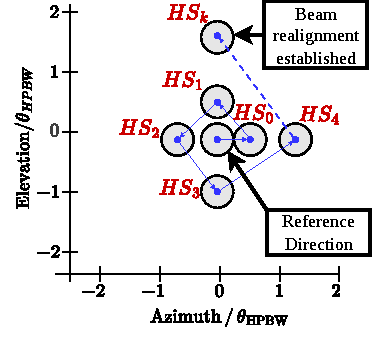
\includegraphics[width=\linewidth]{Figures/Fig9.pdf}
    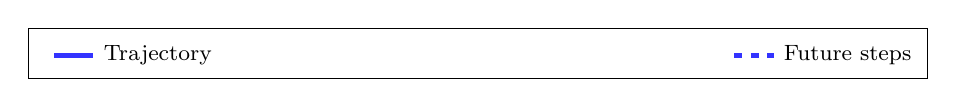
\begin{tikzpicture}
    \node [
            draw=black,
            line width=0.25pt,
            inner sep=3pt,
            rounded corners=0pt,
            align=center
        ] {
            \footnotesize
            \setlength{\tabcolsep}{0pt}
            \renewcommand{\arraystretch}{1.3}
            \begin{tabular*}{\dimexpr0.9\linewidth}{
                c @{\extracolsep{0pt}\hspace{3pt}} l
                @{\extracolsep{\fill}}
                c @{\extracolsep{0pt}\hspace{3pt}} l
            }
                \legline{hs_blue}{solid} & Trajectory &
                \legline{hs_blue}{dashed} & Future steps\\
            \end{tabular*}
        };
    \end{tikzpicture}
    \caption{Hierarchical Search spiral trajectory expanding outward from the reference beam direction with step sizes $HS_0, HS_1, \ldots, HS_k$. Circles show the evaluation order; the scan ends when received power exceeds $P_{\text{succ}}(\Delta t)$.}
    \label{fig:blind_spiral_search}
    \vspace{-5pt}
\end{wrapfigure}
Hierarchical Search operates independently and identically at both the AP and UE. Since the procedure is triggered by link failure, no communication between the nodes is possible during recovery; each node executes its own search using only local power measurements.

The procedure is initiated when a short-term Exponentially Weighted Moving Average (EWMA) of received power drops below a failure threshold $P_{\text{fail}} = P_{\text{ref}} - \Gamma_{\text{fail}}$, where $P_{\text{ref}}$ is the reference power (the last successfully received power level before failure) and $\Gamma_{\text{fail}}$ is the failure margin (parameters in Table~\ref{tab:system_parameters}). Upon detection, each node independently executes a discrete spiral scan outward from its reference beam direction (Fig.~\ref{fig:blind_spiral_search}), adapted from optical alignment systems\cite{photonics11060540} \rev{and consistent with the SSB-based beam search defined for 3GPP NR\cite{Giordani2018ATO, Heng2021SixChallenges}}. The step size for successive rings, $HS_k$, grows exponentially from an initial value proportional to the antenna's HPBW:
\begin{equation}
    HS_k = HS_0 \cdot \gamma^k,
\end{equation}
where $k$ is the ring index, $HS_0 = \theta_{\text{HPBW}}/2$ is the initial step size (half the antenna beamwidth), and $\gamma = 1.25$ is the growth factor. The scan terminates when the received power for a given beam configuration exceeds a time-dependent success threshold $P_{\text{succ}}(\Delta t)$:
\begin{equation}
    P_{\text{succ}}(\Delta t) = P_{\text{ref}} - \Gamma(\Delta t) = P_{\text{ref}} - (\Gamma_{0} + R \cdot \Delta t),
\end{equation}
where $\Gamma_{0}$ is the initial margin, $R$ is the margin increase rate, and $\Delta t$ is the elapsed time since failure detection. The relaxing margin accounts for the growing positional uncertainty: as more time elapses, the node accepts weaker beam configurations to avoid indefinite searching. Once a beam configuration exceeding $P_{\text{succ}}(\Delta t)$ is found, the node holds that beam direction and resumes data exchange.

\subsection*{IMU-Assisted Reactive Search}
\begin{wrapfigure}{r}{0.4\linewidth}
    \centering
    \vspace{-15px}
    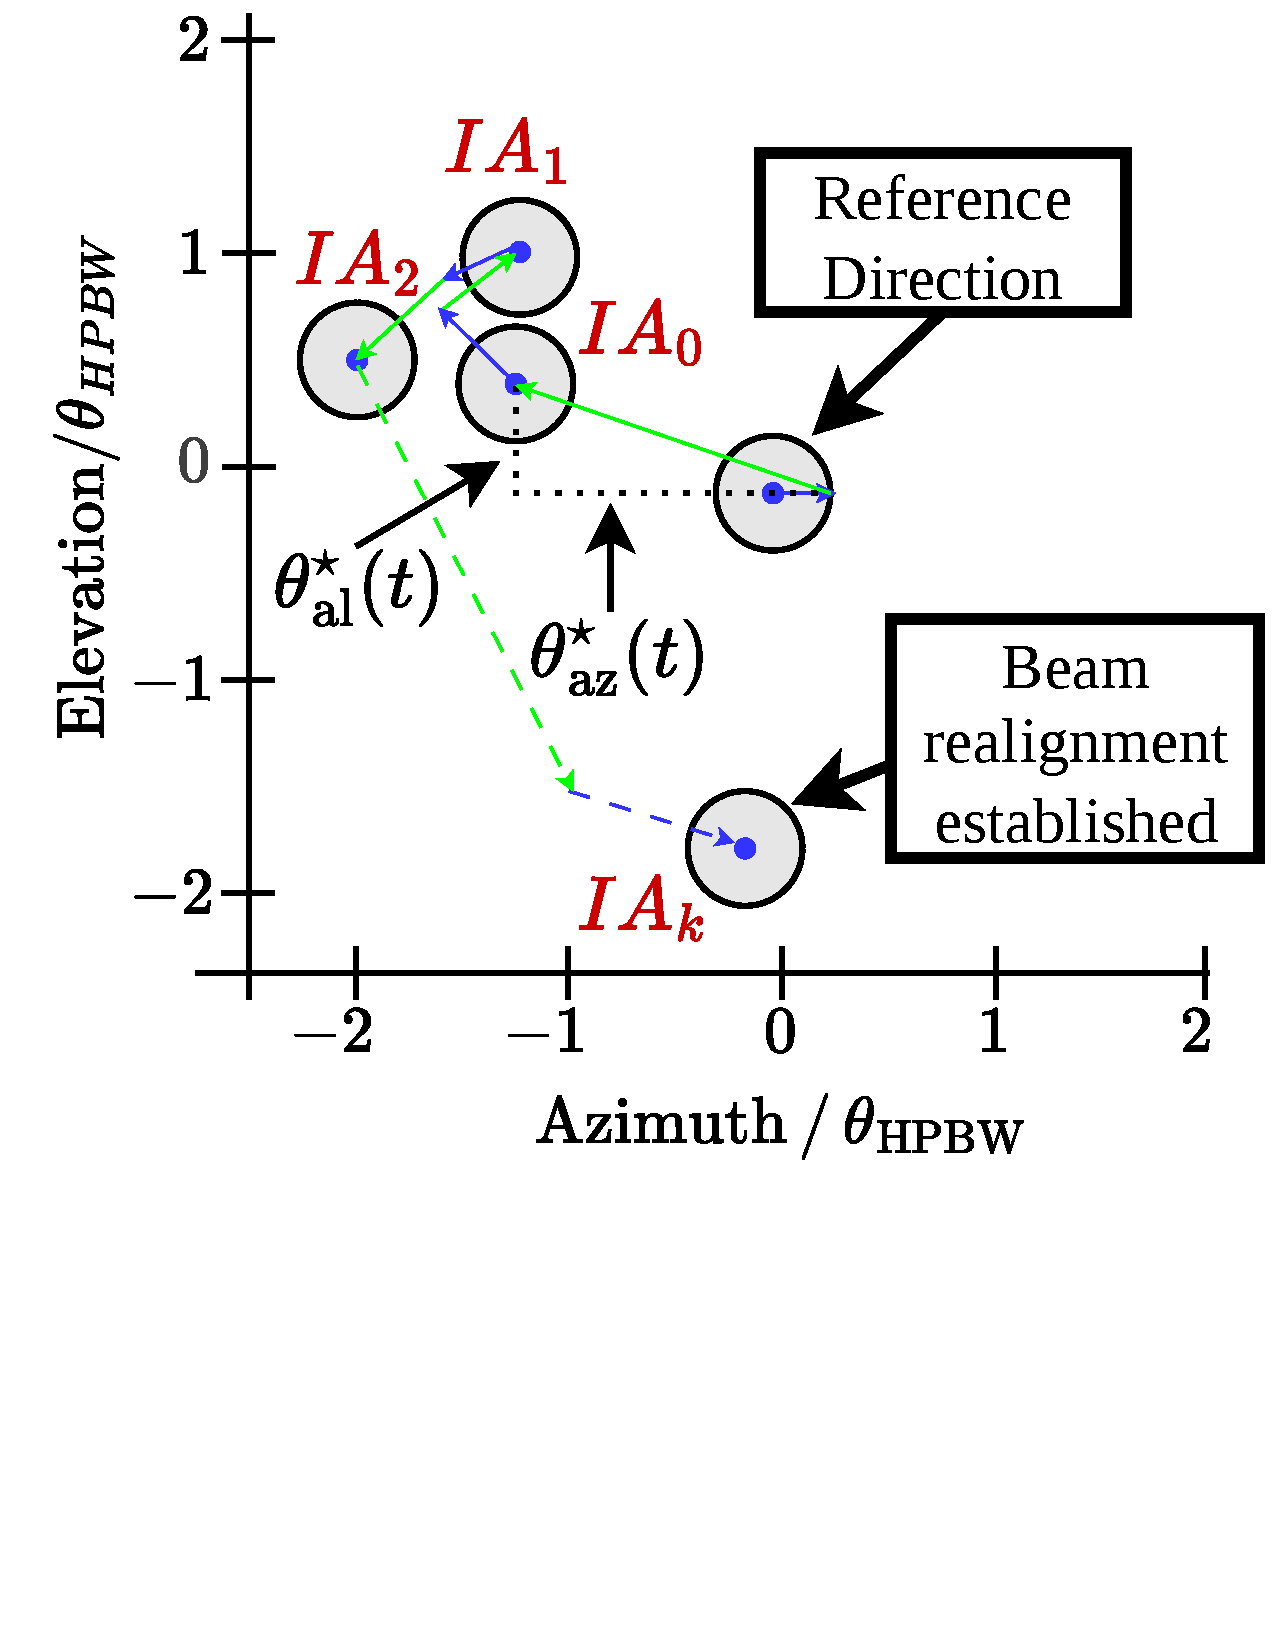
\includegraphics[width=\linewidth]{Figures/Fig10.pdf}\\[-70pt]
    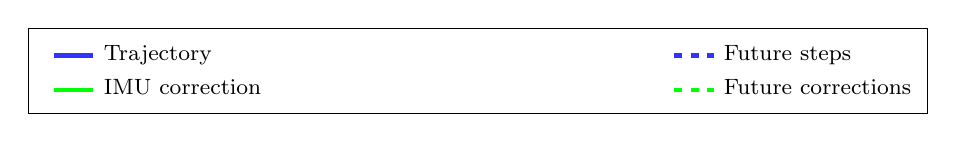
\begin{tikzpicture}
    \node [
            draw=black,
            line width=0.25pt,
            inner sep=3pt,
            rounded corners=0pt,
            align=center
        ] {
            \footnotesize
            \setlength{\tabcolsep}{0pt}
            \renewcommand{\arraystretch}{1.3}
            \begin{tabular*}{\dimexpr0.9\linewidth}{
                c @{\extracolsep{0pt}\hspace{3pt}} l
                @{\extracolsep{\fill}}
                c @{\extracolsep{0pt}\hspace{3pt}} l
            }
                \legline{hs_blue}{solid} & Trajectory &
                \legline{hs_blue}{dashed} & Future steps\\
                \legline{imu_green}{solid} & IMU correction &
                \legline{imu_green}{dashed} & Future corrections\\
            \end{tabular*}
        };
    \end{tikzpicture}\\
    \caption{IMU-Assisted search trajectory. IMU corrections (green) shift the search center to the sensor-predicted LoS direction before each spiral step. The local refinement spiral (blue) scans around the corrected center.}
    \label{fig:imu_local_search}
    \vspace{-5px}
\end{wrapfigure}
The IMU-Assisted algorithm uses the same power-drop trigger as Hierarchical Search but replaces the undirected spiral beam steering trajectory with a refined sensor-directed steering trajectory (Fig.~\ref{fig:imu_local_search}). This procedure is built upon a principle of Kalman-filter-based predictive tracking\cite{8455289,9145366} but operates in a triggered rather than continuous mode. Upon failure detection, the UE integrates accelerometer data into a displacement vector $\Delta\mathbf{p}(t)$ and fuses gyroscope data for orientation change, predicting the new beam pointing direction via:
\begin{equation}
    \theta_{\text{az}}^{\star}(t) = \theta_{\text{az,0}} + \arctan\!\left(\frac{\Delta p_{y}}{\hat{d}_{\text{link}}}\right) + \Delta\psi(t)
\end{equation}
\begin{equation}
    \theta_{\text{el}}^{\star}(t) = \theta_{\text{el,0}} + \arctan\!\left(\frac{\Delta p_{z}}{\hat{d}_{\text{link}}}\right) + \Delta\phi(t)
\end{equation}
where $\theta_{\text{az,0}}$ and $\theta_{\text{el,0}}$ are the last known-good angles; $\Delta p_y$ and $\Delta p_z$ are the horizontal and vertical components of displacement perpendicular to the LoS; $d_{\text{link}}$ is the estimated AP--UE link distance from the last known-good reference time before the link failure; and $\Delta\psi(t)$ and $\Delta\phi(t)$ are the changes in yaw and pitch, respectively. The UE then steers directly to this predicted angle. However, because IMU-based positioning relies on double-integrating noisy accelerometer readings, small measurement errors accumulate over time, causing the estimated position and orientation to progressively diverge from their true values (a phenomenon known as integration drift). To compensate for this residual sensor error, the algorithm follows the predicted steer with a localized refinement phase identical in purpose to the one used by Hierarchical Search but with a tighter step size:
\begin{equation}
    IA_k = \beta \cdot \theta_{\text{HPBW}} + \Delta\theta_{\text{az}}^{\star}(t) + \Delta\theta_{\text{el}}^{\star}(t), \quad (\beta = 0.1)
\end{equation}
Unlike the expanding step size $HS_k$ used in the Hierarchical Search's Search Phase, the base refinement step $\beta \cdot \theta_{\text{HPBW}}$ is fixed and deliberately small (one-tenth of the beamwidth), while the IMU-predicted azimuth and elevation corrections adapt $IA_k$ over time as the sensor estimates evolve. The node scans a tight spiral around the IMU-predicted direction using this step size until an alignment is made (see Fig.~\ref{fig:imu_local_search}). \rev{The reported $\beta = 0.1$ minimizes overshooting at low acceleration while preserving fast convergence at high acceleration.}

%-------------------------------------------------------------------%
\subsection*{JIT Beam Realignment}
While the reactive IMU-Assist algorithm discussed above aims to minimize the beam realignment time once the link failed, our proposed proactive+reactive JIT strives to also prevent the link failure from happening (by realigning the AP and UE beams continuously while the link is still in place). At the same time, not to compromise the actual data exchange and link performance, JIT strives not to produce control signaling overheads and beam re-steering actions unless it is necessary to prevent the link failure. This goal is achieved by designing the system that only triggers beam realignment when the combination of motion speed and link geometry threatens to place the UE outside the AP's beam before the next control cycle.

\rev{\subsubsection*{Trigger Boundary and Edge of Coverage}
The EoC is the angle off the AP's beam axis at which the antenna gain has dropped by \SI{3}{\deci\bel}, i.e., $\theta_{\text{HPBW}}/2$ off boresight. Crossing the EoC corresponds to a worst-case \SI{6}{\deci\bel} round-trip gain loss, particularly punishing in sub-THz where narrow, high-gain beams leave little SNR margin, and can directly cause link failure. Because reaching the EoC under mobility leaves no time for control signaling, JIT instead places a \emph{trigger boundary} inside the EoC, at the offset where the projected displacement during the system reaction time $T_{\text{react}}$ would reach $\eta \cdot \theta_{\text{HPBW}}$. The boundary adapts to motion: as the UE's Link Deviation Velocity $\|\dot{\boldsymbol{\delta}}\|$ (defined below) grows, the projected displacement reaches $\eta \cdot \theta_{\text{HPBW}}$ at a smaller angular offset from boresight, so the trigger fires earlier, farther inside the EoC. When motion slows, the boundary moves outward toward the EoC, suppressing unnecessary control frames. For AP-stationary scenarios (e.g., a wall-mounted access point serving mobile UEs), detection of approaching EoC is performed \emph{locally} at the UE: at every IMU sample, the UE evaluates Eq.~(\ref{eq:trigger}) using its body-frame kinematics and the known $\theta_{\text{HPBW}}$ of its own antenna, requiring no AP-side feedback. In future work, mobile-AP cases (e.g., UAV-borne access points) would extend the protocol so the AP also shares its kinematic state via the same control frame.}

\rev{A stationary Zero Velocity Update (ZUPT) phase is performed at initialization to calibrate the accelerometer bias $\mathbf{b}_a$ and gyroscope bias $\mathbf{b}_\omega$, since any practical IMU has noise that would otherwise propagate into the trigger evaluation. During this phase the UE remains stationary briefly, and the mean of the raw accelerometer and gyroscope readings provides a direct estimate of the sensor biases (true acceleration and angular velocity are both zero). These estimates are then subtracted from all subsequent IMU readings to obtain corrected acceleration $\mathbf{a}_{\text{corr}}[n] = \tilde{\mathbf{a}}[n] - \mathbf{b}_a$ and angular velocity $\boldsymbol{\omega}_{\text{corr}}[n] = \tilde{\boldsymbol{\omega}}[n] - \mathbf{b}_\omega$, separating link-critical motion from sensor noise. Utilizing the corrected IMU data, the UE continuously computes a new metric, the \emph{Link Deviation Velocity} $\dot{\boldsymbol{\delta}}$, which unifies rotational and LoS-perpendicular translational motion into a single angular rate of deviation:}
\begin{equation}
    \dot{\boldsymbol{\delta}} = \boldsymbol{\omega}_{\text{UE}} + \frac{\mathbf{v}_{\perp}}{d_{\text{link}}},
    \label{eq:link_deviation_velocity}
\end{equation}
where $\boldsymbol{\omega}_{\text{UE}}$ is the UE's angular velocity, $\mathbf{v}_{\perp}$ is its translational velocity perpendicular to the LoS, and $d_{\text{link}}$ is the instantaneous link distance. This metric hence serves as a measure of ``how fast the UE movements are approaching the AP beam boundaries''. \rev{Both terms in Eq.~(\ref{eq:link_deviation_velocity}) are expressed in the AP-anchored world coordinate frame: the UE's body-frame angular velocity $\boldsymbol{\omega}_{\text{UE}}$ and translational velocity perpendicular to the LoS, $\mathbf{v}_{\perp}$, are transformed via the UE's orientation quaternion $\mathbf{q}_{\text{body}}$ (the same quaternion that contributes to $\mathbf{q}_{\text{eff}}$ in the antenna pattern evaluation discussed below). This common frame ensures that rotational and LoS-perpendicular translational contributions to beam deviation are summed consistently as a single 3D angular rate.}

\rev{Two design choices bound the residual drift. The trigger condition (Eq.~\ref{eq:trigger}, below) uses the Link Deviation \emph{velocity} rather than an absolute position (single vs double accelerometer integration), and the control frame transmits only the displacement change since the last transmission, with the accumulator reset at each transmission so cumulative drift cannot grow with session length. Over the AP's per-prediction window $T_{\text{react}} \approx \SI{15}{\micro\second}$, the resulting position-prediction drift is bounded by $\sigma_{p} = \sigma_{a,n}\sqrt{T_{\text{react}}^{3}/3} \lesssim \SI{1}{\nano\meter}$ for the noise density in Table~\ref{tab:system_parameters}, an angular drift of order $10^{-8}$~degrees at $d_{\text{link}} = \SI{3}{m}$ and far below $\theta_{\text{HPBW}}$; across longer tracking sessions the accumulator reset bounds cumulative drift by a single inter-transmission interval rather than the full session duration. JIT specifically targets this initial, unpredictable phase of motion. For sustained continuous-mobility scenarios (e.g., a pedestrian walking continuously, or a vehicle in steady transit), complementary bias-tracking from the inertial-navigation literature such as learning-based dead-reckoning~\cite{Brossard2020AIIMU}, deep-learning drift compensation~\cite{Chen2024DLInertial}, or zero-velocity detection~\cite{Skog2010ZUPT} would augment JIT's calibration as future work.}

Finally, a control frame is triggered when the projected angular displacement over the system's reaction time $T_{\text{react}}$ exceeds a fraction $\eta$ of the antenna's HPBW:
\begin{equation}
    \|\dot{\boldsymbol{\delta}}\| \cdot T_{\text{react}} > \eta \cdot \theta_{\text{HPBW}}
    \rev{\label{eq:trigger}}
\end{equation}
The guard fraction $\eta$ trades off link robustness against control overhead: a lower $\eta$ triggers control frames earlier, providing more margin against sudden motion at the cost of higher signaling frequency, while a higher $\eta$ reduces overhead but leaves less time to react before the beam exits the main lobe. We use $\eta = 0.36$ across our evaluated scenarios; \rev{mean capacity stays within \SI{5}{\percent} of its maximum across $\eta \in [0.25, 0.50]$, where the lower end fires earlier with more signaling overhead and the upper end fires later with less reaction margin, indicating a gradual plateau around the chosen value. The cooldown between consecutive triggers is set to one IMU sampling period to prevent redundant firings within a single sensor cycle.}

Upon triggering, the UE transmits a control frame containing its integrated displacement vector and a buffer of recent IMU samples. \rev{The AP derives a filtered acceleration trend $\bar{\mathbf{a}}_{\text{predict},k}$ from the buffered samples via an EWMA,
\begin{equation}
    \bar{\mathbf{a}}_{\text{predict},k} = \alpha_{\text{short}}\, \mathbf{a}_k + (1 - \alpha_{\text{short}})\, \bar{\mathbf{a}}_{\text{predict},k-1},
    \label{eq:ewma_predict}
\end{equation}
with $\alpha_{\text{short}} = 0.90$ as listed in Table~\ref{tab:system_parameters}. This low-pass cutoff suppresses high-frequency IMU sensor noise while preserving the underlying acceleration trend, and the AP then extrapolates the UE's position at steering completion using $\bar{\mathbf{a}}_{\text{predict},k}$.} By steering to this predicted future location rather than the last known position, the system maintains SNR continuity despite rapid motion.

Each control frame follows the IEEE~802.15.3d THz-SC structure\cite{9269931}, using a short Preamble Acquisition Preamble (PAP) of \SI{1.89}{\micro\second} and the minimum 2048-byte frame payload. With worst-case BPSK modulation and 11/15 LDPC coding, each control frame occupies approximately $T_{\text{frame}} \approx \SI{5}{\micro\second}$. The end-to-end reaction latency comprises the control frame transmission time ($T_{\text{frame}}$) and the AP's signal acquisition and processing delay ($T_{\text{proc}} = \SI{10}{\micro\second}$), giving a total signaling latency of $T_{\text{react}} = T_{\text{frame}} + T_{\text{proc}} \approx \SI{15}{\micro\second}$ before the AP can issue a steering command. \rev{The IMU sampling period (\SI{10}{\milli\second} in this evaluation; commodity $\geq$\SI{1}{\kilo\hertz} IMUs such as the Bosch BMI270 are widely available) gates only the rate at which Eq.~(\ref{eq:trigger}) is evaluated; once a trigger fires, the control-frame transmission, AP processing, and steering actuation all proceed on their own clocks, decoupled from the IMU sample interval.}

Reliable decoding at the AP requires a minimum receive SNR of \SI{9.59}{\deci\bel}, corresponding to BPSK with 11/15 LDPC coding at a target $\text{BER} = 10^{-3}$. \rev{This SNR threshold also doubles as an RF-side fallback trigger:} if the instantaneous SNR falls below \SI{9.59}{\deci\bel}, the AP cannot decode the control frame and the system falls back to reactive recovery, with the UE continuing to steer using its local IMU data while the AP, lacking motion awareness, initiates a Hierarchical Search to restore alignment. \rev{Motion fast enough to outpace IMU-based prediction without already producing RF-side degradation is rare in practice (typical human-scale or vehicular motion develops over tens to hundreds of IMU samples, i.e., hundreds of milliseconds to seconds, well within the IMU detection window), so the IMU + RF combination provides defense in depth across realistic operating regimes.}




%-------------------------------------------------------------------%
\subsection*{The MobileTHz Simulation Platform}
The MobileTHz platform discretizes time into fixed-duration slots of length $\Delta t_{\text{sim}} = \SI{1}{\micro\second}$, enabling deterministic, slot-by-slot evaluation of node kinematics, RF channel state, hardware behavior, and algorithm decisions. Simulation parameters, listed in Table~\ref{tab:system_parameters}, mirror the experimental hardware properties to ensure close correspondence between simulated and measured results.

\begin{table}[ht]
\centering
\small
\caption{Shared system parameters for the channel model, transceiver, IMU sensor, and beam-management algorithms. All values are common to the three steering configurations.}
\label{tab:system_parameters}
\sisetup{per-mode=symbol}
\begin{tabularx}{\linewidth}{@{}Xr@{\hskip 12pt}Xr@{}}
\toprule
\textbf{Parameter} & \textbf{Value} & \textbf{Parameter} & \textbf{Value} \\
\midrule
\multicolumn{2}{@{}l}{\textbf{\textit{Channel}}} & \multicolumn{2}{@{}l}{\textbf{\textit{IMU Sensor}}} \\
\cmidrule(r){1-2} \cmidrule(l){3-4}
Carrier Frequency ($f_c$) & \SI{130}{\giga\hertz} & Gyro.\ Noise Density & \SI{0.00175}{\radian\per\second\per\sqrt{\hertz}} \\
Bandwidth ($B$) & \SI{8}{\giga\hertz} & Accel.\ Noise Density & \SI{0.0294}{\meter\per\second\squared\per\sqrt{\hertz}} \\
System Temperature ($T$) & \SI{290}{\kelvin} & Initial Bias Std.\ Dev. & \num{0.01} (gyro/accel) \\
Thermal Noise ($k_B T B$) & \SI{-75.0}{dBm} & Sampling Period & \SI{10}{\milli\second} \\[3pt]
\multicolumn{2}{@{}l}{\textbf{\textit{Transceiver}}} & \multicolumn{2}{@{}l}{\textbf{\textit{Algorithm Parameters}}} \\
\cmidrule(r){1-2} \cmidrule(l){3-4}
Tx Power ($P_{tx}$) & \SI{13}{dBm} & Failure Margin ($\Gamma_{\text{fail}}$) & \SI{3}{\deci\bel} rel.\ $P_{\text{ref}}$ \\
Rx Noise Factor ($F$) & 14.83 (\SI{11.7}{\deci\bel}) & EWMA Coeff.\ ($\alpha_{\text{short}}$) & 0.90 \\
Rx Processing Delay ($T_{\text{proc}}$) & \SI{10}{\micro\second} & Spiral Growth Factor ($\gamma$) & 1.25 \\
& & Initial Success Margin ($\Gamma_0$) & \SI{0.25}{\deci\bel} \\
& & Margin Increase Rate ($R$) & $0.5 \cdot G_{\max}$~dB/s \\
\bottomrule
\end{tabularx}
\end{table}

A mobile scenario consists of a set of mobile nodes, $\mathcal{M} = \{m_1, m_2, \dots\}$, whose trajectories are specified by a sequence of keyframes, $\{(\mathbf{p}_k, \mathbf{q}_k)\}_{k=0}^{K-1}$. Each keyframe defines the position $\mathbf{p}_k \in \mathbb{R}^3$ and orientation (as a unit quaternion) $\mathbf{q}_k \in \mathbb{S}^3$ at a specific time slot $n_k$. To create smooth and realistic translational paths between keyframes, the platform interpolates position using Perlin's smootherstep function\cite{Perlin2002}, $f(\tau)$:
\begin{equation}
f(\tau) = 6\tau^5 - 15\tau^4 + 10\tau^3,
\label{eq:smootherstep}
\end{equation}
where $\tau = (t - t_k) / (t_{k+1} - t_k) \in [0, 1]$ is the normalized time. This function's $C^2$ continuity guarantees zero velocity, acceleration, and jerk at keyframe boundaries, producing physically plausible motion. \rev{The zero-velocity boundary condition models pause-resume mobility patterns such as walking with intermediate stops or beginning and ending a turn from rest, which are the primary motion classes considered in this study. Both the software simulator and the HIL testbed natively support trajectories without a stationary boundary (e.g., continuous walking through multiple checkpoints) by chaining smootherstep-interpolated segments whose endpoints exchange non-zero velocities, preserving slot-by-slot $C^1$ continuity where required.}

\rev{For a single smootherstep segment,} the maximum acceleration \rev{produced by Eq.~\eqref{eq:smootherstep}} over a displacement $D$ \rev{and} duration $T$ is:
\begin{equation}
    a_{\max} = K \cdot \frac{D}{T^2},
\end{equation}
where $K \approx 5.7735$ is derived from the peak of the second derivative of Eq.~\eqref{eq:smootherstep}. Orientation, in turn, is interpolated via Spherical Linear Interpolation (SLERP)\rev{\cite{Shoemake1985SLERP}}:
\begin{equation}
    \text{SLERP}(\mathbf{q}_k, \mathbf{q}_{k+1}, \tau) = \frac{\sin((1-\tau)\Theta)}{\sin\Theta}\mathbf{q}_k + \frac{\sin(\tau\Theta)}{\sin\Theta}\mathbf{q}_{k+1},
\end{equation}
where $\Theta = \arccos(\mathbf{q}_k \cdot \mathbf{q}_{k+1})$. Translational and angular velocities and accelerations are obtained via central finite differences of position and orientation, respectively.

Given the updated node kinematics, the engine evaluates the RF link state. Free-space path loss (FSPL), $L_p$, in dB is:
\begin{equation}
    L_{p} = 20 \log_{10}(d_{\text{link}}) + 20 \log_{10}(f_c) - 147.55,
\end{equation}
where $d_{\text{link}} = ||\mathbf{p}_{rx} - \mathbf{p}_{tx}||$ is the instantaneous LoS distance in meters and $f_c$ is the carrier frequency in Hz. Antenna directivity is evaluated from the node's effective orientation $\mathbf{q}_{eff} = \mathbf{q}_{body} \otimes \mathbf{q}_{rotary}$, which transforms the LoS vector into the antenna's local frame to obtain the off-axis angle. The directivity follows the E-plane pattern of a WR-6.5 conical horn, whose gain $G(\theta)$ is given by:
\begin{equation}
    G(\theta) = \frac{1 + \cos(\theta)}{2} \sqrt{\frac{(C(r_2) - C(r_1))^2 + (S(r_2) - S(r_1))^2}{4(C(r_0)^2 + S(r_0)^2)}},
\end{equation}
where $C(x)$ and $S(x)$ are the Fresnel cosine and sine integrals with arguments:
\begin{equation}
    r_0 = \frac{b_\mathrm{wg}}{2}\sqrt{\frac{\beta_g}{\pi R_h}}, \quad
    r_{1,2} = \sqrt{\frac{\beta_g}{\pi R_h}}\left(\mp\frac{B_E}{2} - \frac{R_h \beta_g B_E}{2}\sin\theta\right),
    \beta_g = \frac{2\pi}{\lambda}\sqrt{1-\left(\frac{\lambda}{2a_\mathrm{wg}}\right)^2}
\end{equation}
Here $R_h = \SI{25}{\milli\meter}$ is the horn slant length, $B_E = \SI{3.59}{\milli\meter}$ is the effective E-plane aperture, $b_\mathrm{wg} = \SI{0.826}{\milli\meter}$ and $a_\mathrm{wg} = \SI{1.651}{\milli\meter}$ are the waveguide height and width, respectively. Then, the maximum gain is defined as $G_\mathrm{max} = \max_{\theta} G(\theta)$. \rev{For 3D evaluation, the radiation pattern is treated as rotationally symmetric about the boresight: the gain $G(\theta)$ depends only on the off-axis angle $\theta$ obtained by transforming the 3D LoS vector into the antenna's local frame via $\mathbf{q}_{\text{eff}}$, and the E-plane formula above is applied across all azimuth angles around boresight as a rotationally symmetric approximation. The HIL measurements cross-check this approximation against the physical horn and confirm that it is sufficient for this evaluation.} The received power (in dBm) then combines transmit power, directional gains, and path loss:
\begin{equation}
P_{rx} = P_{tx} + G_{tx}(\theta_{tx}) + G_{rx}(\theta_{rx}) - L_p,
\end{equation}
where $P_{tx}$ is the transmit power and $\theta_{tx}$, $\theta_{rx}$ are the off-axis angles at the transmitter and receiver, respectively.

The simulation then applies a hardware abstraction layer that models the constraints of physical components. A steerable antenna's orientation is controlled by a dual-axis mechanical stage, which adjusts the $\mathbf{q}_{rotary}$ component of the effective orientation. For any instructed angular displacement $\Delta\theta$, the model uses a trapezoidal velocity profile:
\begin{equation}
	a(t) =
	\begin{cases}
		+\alpha_{\text{max}} & \text{Phase I: Acceleration}       \\
		0               & \text{Phase II: Constant velocity} \\
		-\alpha_{\text{max}} & \text{Phase III: Deceleration}     \\
	\end{cases},
\end{equation}
where the duration of each phase is determined by $\Delta\theta$, the stage's maximum angular velocity, $\omega_{max}$, and the angular acceleration constraints, $\alpha_{max}$.

Beyond mechanical steering, the hardware abstraction layer captures two additional sources of latency and noise. A configurable processing delay $T_{\text{proc}}$ models signal acquisition and digital conversion latency, holding the power reading constant at the value sampled at the start of the previous processing interval. The simulated IMU provides gyroscope ($\boldsymbol{\omega}$), accelerometer ($\mathbf{f}$), and magnetometer data, with realistic outputs generated by corrupting ground-truth kinematics with bias and noise. Denoting the discrete time-slot index by $n$, the simulated accelerometer output $\tilde{\mathbf{a}}[n]$ is:
\begin{equation}
    \tilde{\mathbf{a}}[n] = \mathbf{f}_{ideal}[n] + \mathbf{b}_{a}[n] + \mathbf{n}_{a}[n].
\end{equation}
The bias $\mathbf{b}_{a}[n]$ evolves as a random walk: $\mathbf{b}_{a}[n] = \mathbf{b}_{a}[n-1] + \mathbf{w}_{b,a}[n]$, where the update term $\mathbf{w}_{b,a} \sim \mathcal{N}(0, \sigma_{a,b}^2 \Delta t_{\text{sim}} \cdot \mathbf{I}_3)$ and the white noise is $\mathbf{n}_{a}[n] \sim \mathcal{N}(0, (\sigma_{a,n}^2 / \Delta t_{\text{sim}}) \cdot \mathbf{I}_3)$. A similar noise model is applied to the gyroscope readings. The noise density parameters $\sigma_{a,n}$ and bias random walk parameter $\sigma_{a,b}$ correspond to the Accelerometer Noise Density and Initial Bias values in Table~\ref{tab:system_parameters}, respectively.

This sequence of kinematics update, channel evaluation, hardware emulation, and algorithm decision repeats at every \SI{1}{\micro\second}-long time slot, producing the continuous per-slot feedback loop that drives all simulated results in this article.

%-------------------------------------------------------------------%
\subsection*{The Experimental Platform}
A similar per-slot loop calculation procedure works in the HIL mode, employing the hardware sub-THz platform. However, the simulated RF and sensor inputs discussed in the previous subsection get replaced by actual physical measurements. Specifically, the received power data comes from the RF hardware, orientation data gets fetched from rotary-stage encoders, and inertial data from an on-device IMU. The complete testbed is illustrated in Fig.~\ref{fig1_algorithms}.

\begin{figure}[t]
\centering
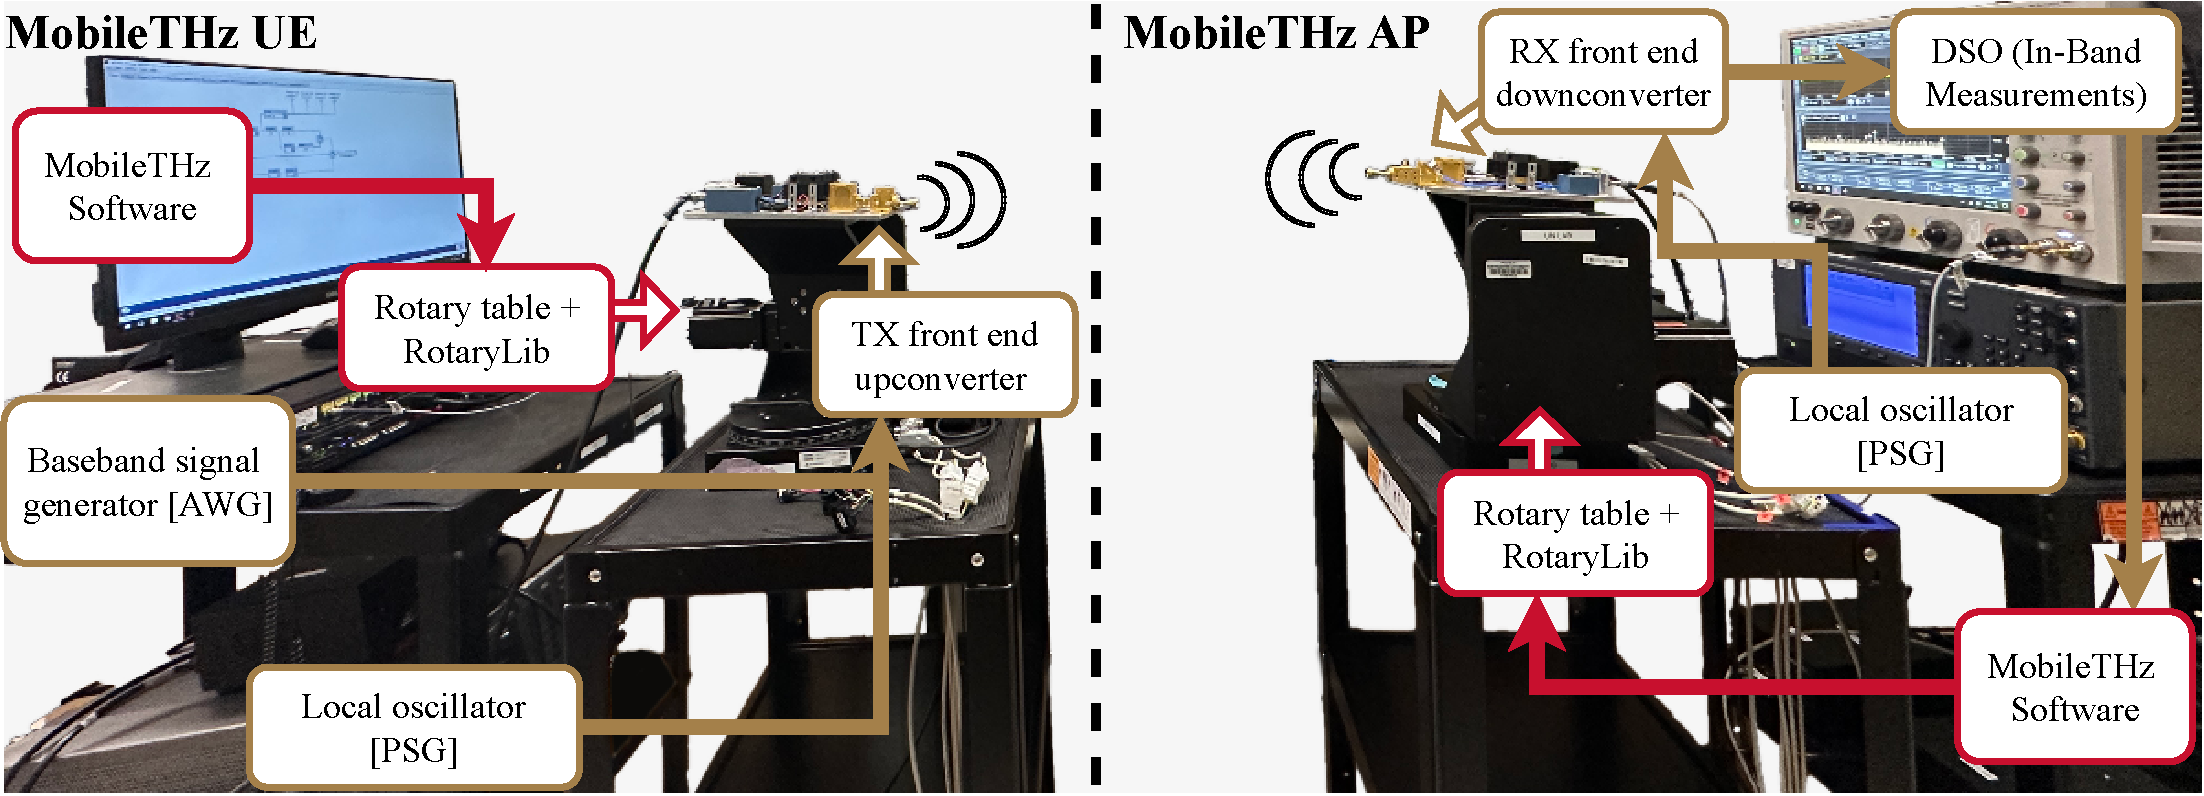
\includegraphics[width=\linewidth]{Figures/Fig11.pdf}
\caption{MobileTHz HIL testbed. The UE (left) and AP (right) each pair a sub-THz RF front-end with a dual-axis rotary stage. A 9-axis IMU on the UE supplies inertial data for the IMU-Assisted and JIT algorithms.}
\label{fig1_algorithms}
\vspace{-5pt}
\end{figure}

The RF chain operates in the WR-6.5 waveguide band (110--170~GHz). On the transmit side, a Keysight E8257D PSG and M8196A AWG feed a VDI MixAMC upconverter; on the receive side, a VDI MixAMC downconverter and Keysight DSOZ632A oscilloscope capture in-band power. Each front-end is mounted on an IntelLiDrives dual-axis rotary table equipped with a VDI WR-6.5 conical horn antenna (\SI{21}{dBi}, \SI{13}{\degree} HPBW). A WitMotion WT901BLECL 9-axis IMU, co-located with the UE front-end, supplies the inertial data used by the IMU-Assisted and JIT algorithms.

A custom in-house-developed C++ library (RotaryLib) controls the rotary table movements by sending commands via serial connection. Each commanded motion follows the same trapezoidal acceleration-cruise-deceleration profile assumed by the simulator, ensuring that physical stage behavior matches the simulated steering model. Power measurements, encoder feedback, and IMU samples are streamed back to the MobileTHz engine, allowing the same beam management algorithm code to run on physical data without modification.



%-------------------------------------------------------------------%
\subsection*{Evaluation Metrics}
We evaluate the proposed beam management algorithms across four Key Performance Indicators (KPIs) derived from the RF and mobility parameters summarized in Table~\ref{tab:system_parameters} and Table~\ref{tab:steering_and_hardware}. They complement each other, allowing us to evaluate the performance and reliability of various beam realignment strategies from different perspectives.

\emph{Mean Link Capacity} serves as the primary performance metric, calculated as the time-average of instantaneous Shannon capacity $C(t)$ over the duration of the scenario $T$:
\begin{equation}
    \bar{C} = \frac{1}{T} \int_{0}^{T} B \log_2(1 + \text{SNR}(t)) \, dt
\end{equation}
where $B$ represents the channel bandwidth. However, as the link is not always available due to beam misalignment, the calculated mean capacity also obscures the impact of beam misalignment and outages on higher-layer protocols (e.g., TCP).

The second metric of interest in our study is the Capacity CoV, used to quantify the capacity variance over time.
To compute the CoV, we normalize the standard deviation of capacity ($\sigma_C$) by its mean ($\mu_C$):
\begin{equation}
    \text{CoV} = \frac{\sigma_C}{\mu_C}
\end{equation}
High CoV values indicate erratic tracking and jitter, whereas lower values approaching zero indicate a more stable and reliable link.

To further assess the operational feasibility of the link for actual data transmission, we then evaluate \emph{Link Availability ($A_{\text{link}}$}. This metric measures the fraction of time the link budget is sufficient to support high-order modulation schemes, specifically where the $\text{SNR}(t)$ exceeds a critical threshold $\text{SNR}_{\text{th}}$:
\begin{equation}
    A_{\text{link}} = \frac{1}{T} \int_{0}^{T} \mathbbm{1}\!\left(\text{SNR}(t) \geq \text{SNR}_{\text{th}}\right) dt \times 100\%
\end{equation}

The threshold $\text{SNR}_{\text{th}} = \SI{18.8}{\deci\bel}$ corresponds to 64-QAM at a FEC $\text{BER} = 10^{-3}$, derived from the standard $M$-QAM approximation\cite{Proakis2008}:
\begin{equation}
    \text{SNR}_{\text{th}} \approx \frac{M-1}{3} \left[ Q^{-1} \left( \frac{\text{BER}_{\text{target}} \cdot \log_2 M}{4} \right) \right]^2
\end{equation}
which evaluates to \SI{18.8}{\deci\bel}.

Last but not least, we also quantify the bandwidth cost (overheads) of JIT's additional control frames via Signaling Overhead ($O_{\text{sig}}$). The rationale here is to provide a fair evaluation, since the link cannot carry any user data during each control frame transmission. Hence, while the JIT-imposed additional link robustness contributes to the channel capacity and availability, this comes at a cost of additional signaling overhead that has to be carefully estimated.

The foregone capacity over $N_{\text{pp}}$ transmissions is:
\begin{equation}
    L_{\text{ctrl}} = \sum_{i=1}^{N_{\text{pp}}} C(t_i) \cdot T_{\text{frame}},
\end{equation}
where $C(t_i)$ is the instantaneous capacity at the $i$-th transmission and $T_{\text{frame}}$ is the control frame duration derived in the JIT Algorithm subsection. Signaling overhead is then:
\begin{equation}
    O_{\text{sig}} = \frac{L_{\text{ctrl}}}{\int_{0}^{T} C(t) \, dt} \times 100\%
\end{equation}

While the considered beam realignment strategies can, in principle, be evaluated in our platform across multiple other metrics, the selected set of four diverse KPIs already present a comprehensive view on the key trade-offs.

%-------------------------------------------------------------------%
\subsection*{Statistics and Reproducibility}
All comparisons between algorithms are based on deterministic metrics (Mean Capacity, Capacity CoV, Link Availability, Signaling Overhead) computed over the full scenario duration for each configuration. All percentage improvements reported between algorithms (e.g., ``JIT achieves up to an 88\% improvement over IMU-Assist'') are computed directly from the respective mean capacity or link availability values at matched operating points. These comparisons reflect differences in algorithmic design evaluated under identical controlled conditions.

Each simulation data point averages $n = 5{,}000$ independent Monte Carlo runs. The source of randomness depends on the scenario: in translational cases, the UE movement direction is drawn uniformly from $[0, 2\pi)$ with no rotation; in rotational cases, the rotation sense and axis are randomized with no translation; in combined-motion cases, both direction and rotation are randomized; and in link-geometry sweeps, the motion profile is fixed while the geometric parameter (separation distance or angular displacement) is varied deterministically. All other parameters (carrier frequency, transmit power, antenna configuration, steering model) are kept constant within each sweep as specified in Tables~\ref{tab:steering_and_hardware} and~\ref{tab:system_parameters}.

Each experimental (HIL) data point averages $n = 10$ independent measurement trials. \rev{The dual-axis rotary stages support full 3D antenna pointing in both azimuth and altitude; the linear translation of the RF front-end mounts, however, was constrained to the azimuth plane by the weight of the RF equipment.} Agreement between simulation and experiment is quantified using MAPE and NRMSE, computed as:
\begin{equation}
    \text{MAPE} = \frac{1}{N} \sum_{i=1}^{N} \left| \frac{\bar{C}_{\text{sim},i} - \bar{C}_{\text{exp},i}}{\bar{C}_{\text{sim},i}} \right| \times 100\%
\end{equation}
\begin{equation}
    \text{NRMSE} = \frac{\sqrt{\frac{1}{N}\sum_{i=1}^{N}(\bar{C}_{\text{sim},i} - \bar{C}_{\text{exp},i})^2}}{\bar{C}_{\text{sim,max}} - \bar{C}_{\text{sim,min}}} \times 100\%
\end{equation}
where $\bar{C}_{\text{sim},i}$ and $\bar{C}_{\text{exp},i}$ are the simulated and experimental mean capacities at the $i$-th acceleration point, $N$ is the number of acceleration points in the sweep, and $\bar{C}_{\text{sim,max}}$ and $\bar{C}_{\text{sim,min}}$ are the maximum and minimum simulated mean capacities across the sweep.

%-------------------------------------------------------------------%
%-------------------------------------------------------------------%
%-------------------------------------------------------------------%
\section*{Data Availability}
All data generated or analysed during this study are included in this published article and its supplementary information files. Additional data can be made available to readers upon reasonable request to the corresponding author.

%-------------------------------------------------------------------%
%-------------------------------------------------------------------%
%-------------------------------------------------------------------%
\section*{Code Availability}
Code is publicly available at \url{https://doi.org/10.5281/zenodo.18675630}.

%-------------------------------------------------------------------%
%-------------------------------------------------------------------%
%-------------------------------------------------------------------%
\section*{Acknowledgements}
The work has been supported in part by U.S. National Science Foundation (NSF) projects 2225590 and 2346487, by Digital Futures at KTH, and by the Future Research Leaders program (FFL-9) from the Swedish Foundation for Strategic Research (SSF).

%-------------------------------------------------------------------%
%-------------------------------------------------------------------%
%-------------------------------------------------------------------%
\section*{Author Contributions Statement}
S.P. and V.P. formulated experiments. S.P. performed experiments. S.P. and V.P. analyzed the results. J.J. supervised and directed the project. All the authors contributed to writing the manuscript.

%-------------------------------------------------------------------%
%-------------------------------------------------------------------%
%-------------------------------------------------------------------%
\section*{Competing Interests Statement}
The authors declare no competing interests.

%-------------------------------------------------------------------%
%-------------------------------------------------------------------%
%-------------------------------------------------------------------%
\bibliography{references}

\end{document}
